%%%%%%%%%%%%%%%%%%%% book.tex %%%%%%%%%%%%%%%%%%%%%%%%%%%%%

\documentclass[english, 11pt]{book}

% Some specific typographic conventions used in Griffiths I2QM   START 
\usepackage{mathtools}			% equation tag with [..] instead of (..)
\mathtoolsset{showonlyrefs}     % only tag equations which are \label'ed   <<<<<<  N E W  
\newtagform{brackets}{[}{]}		% equation tag with [..] instead of (..)
\usetagform{brackets}			% equation tag with [..] instead of (..)
\mathtoolsset{showonlyrefs}
% Some specific typographic conventions used in Griffiths I2QM   END 

\usepackage{babel}
% choose options for [] as required from the list
% in the Reference Guide, Sect. 2.2

\usepackage{makeidx}         % allows index generation
\usepackage{graphicx}        % standard LaTeX graphics tool
                             % when including figure files
\usepackage{multicol}        % used for the two-column index
\usepackage[bottom]{footmisc}% places footnotes at page bottom
% etc.
% see the list of further useful packages
% in the Reference Guide, Sects. 2.3, 3.1-3.3
\usepackage[normalem]{ulem}

\usepackage[shortlabels]{enumitem}	% to be able to resume enumerated lists

\usepackage{amsmath}	% To be able to slash
\usepackage{amsfonts}	% To be able to use \mathbb ... 
\usepackage{amssymb}	% To be able to use \nmid ... 
\usepackage{amsthm}		% \qed, \qedhere
\usepackage{slashed}	% any character (dirac)
% Physics package 
% https://tex.stackexchange.com/questions/38978/how-can-i-manually-install-a-latex-package-debian-ubuntu-linux
\usepackage{physics}	
\usepackage[title,toc,page]{appendix}

% To put accents below letters
\usepackage{accents}
% To write two equations side by side
\usepackage{multicol}

% To use PGF/TikZ https://tex.stackexchange.com/questions/3622/best-way-to-generate-nice-function-plots-in-latex
\usepackage{tikz}
\usetikzlibrary{datavisualization}
\usetikzlibrary{datavisualization.formats.functions}

% Force chapter numbering to restart within each part
\makeatletter
%\@addtoreset{chapter}{part}
\makeatletter


\makeindex             % used for the subject index
                       % please use the style svind.ist with
                       % your makeindex program


%%%%%%%%%%%%%%%%%%%%%%%%%%%%%%%%%%%%%%%%%%%%%%%%%%%%%%%%%%%%%%%%%%%%%

\begin{document}

\newcommand{\quotes}[1]{``#1''}
\newcommand{\sfT}{$\mathsf{T}$}
\newcommand{\udT}{\rotatebox[origin=c]{180}{$\mathsf{T}$}}
\newcommand{\N}{\mathbb{N}}
\newcommand{\Z}{\mathbb{Z}}
\newcommand{\Q}{\mathbb{Q}}
\newcommand{\R}{\mathbb{R}}
\newcommand{\C}{\mathbb{C}}

% To put accents below letters. Here \form{\theta} put a tilde below 
\newcommand{\ut}[1]{\underaccent{\tilde}{#1}}
\newcommand{\uh}[1]{\underaccent{\hat}{#1}}
\newcommand{\form}[1]{\uh{#1}}

% To create italic, bold, bolditalic text
\newcommand{\tit}[1]{\textit{#1}}
\newcommand{\tbf}[1]{\textbf{#1}}
\newcommand{\tbi}[1]{\textit{\textbf{#1}}}


\DeclareRobustCommand{\rchi}{{\mathpalette\irchi\relax}}
\newcommand{\irchi}[2]{\raisebox{\depth}{$#1\chi$}} % inner command, used by \rchi

%----------------------------------------------------------------------------------------
%   r Griffiths, curls and fonts from mt2pro[lite]->pro
%----------------------------------------------------------------------------------------
%\def\rcurs{s}
%\def\brcurs{\vb{\rcurs}}
%\def\hrcurs{\vu{\rcurs}}


\author{Marcello Vitaletti}
\title{Notes on the Classical Theory of Fields\\
{\small }}
\maketitle

\frontmatter%%%%%%%%%%%%%%%%%%%%%%%%%%%%%%%%%%%%%%%%%%%%%%%%%%%%%%

%\include{dedic}

%\chapter*{Plan}
\label{plan} 

In this book I am keeping notes about the theory of classical electromagnetism, 
as exposed in various books. In particular, I intend to cover the following materials:

\begin{itemize}

\item B. Felsager -- Geometry Particles and Fields
\begin{enumerate}
\setcounter{enumi}{0}
\item Electromagnetism (1.1 to 1.4)
\end{enumerate}

\item C. Cattaneo -- Teoria Einsteniana della Gravitazione
\begin{enumerate}
\setcounter{enumi}{0}
\item Elementi di Algebra e Analisi Lineare
\end{enumerate}

\item D.J. Griffiths -- Introduction to Electrodynamics
\begin{enumerate}
\setcounter{enumi}{0}
\item Vector Analysis
\item Electrostatics
\item Potentials
\item Electric Fields in Matter
\item Magnetostatics
\item Magnetic Fields in Matter
\item Electrodynamics
\item Conservation Laws
\item Electromagnetic Waves
\item Radiation
\item Electrodynamics and Relativity
\item Potentials and Fields
\item Helmoltz Theorem
\end{enumerate}

\item J.D. Jackson -- Classical Electrodynamics, 2nd Edition
\begin{enumerate}
\setcounter{enumi}{0}
\item Introduction to Electrostatics
\item Boundary Value Problems in Electrostatics - I
\item Boundary Value Problems in Electrostatics - II
\item Multipoles, Electrostatics of Macroscopic Media, Dielectrics
%\item Magnetostatics
%\item Time Varying Fields, Maxwell Equations, Conservation Laws
%\item Plane Electromagnetic Waves and Wave Propagation
%\item Wave Guides and Resonant Cavities
%\item Simple Radiating Systems, Scattering and Diffraction
%\item Magnetohydrodynamics and Plasma Physics
\end{enumerate}

\item J.D. Jackson -- Classical Electrodynamics, 3rd Edition
\begin{enumerate}
\setcounter{enumi}{4}
\item Magnetostatics, Faraday's Law, Quasi-Static Fields
\item Maxwell Equations, Macroscopic Electromagnetism, Conservation Laws
\item Plane Electromagnetic Waves and Wave Propagation
\item Wave Guides, Resonant Cavities and Optical Fibers
\item Radiating Systems, Multipole Fields and Radiation
\item Scattering and Diffraction
\item Special Theory of Relativity
\item Dynamics of Relativistic Particles and Electromagnetic Fields
\end{enumerate}

\item B. Felsager -- Geometry Particles and Fields
% Contacts with quantum theory of particles dynamics in EM fields
\begin{enumerate}
\setcounter{enumi}{1}
\item Interaction of Fields and Particles
\end{enumerate}

\item J. Franklin -- Advanced Mechanics and General Relativity
\begin{enumerate}
\setcounter{enumi}{1}
\item Relativistic Mechanics
\item Tensors
\item Curved Space
\item Scalar Field Theory
\item Tensor Field Theory (6.1 to 6.5)
\end{enumerate}

\item J.D. Jackson -- Classical Electrodynamics, 3rd Edition
\begin{enumerate}
\setcounter{enumi}{12}
\item Collisions, Energy Loss and Scattering of Charged Particles, Cherenkov and Transition Radiation
\item Radiation by Moving Charges
\item Bremsstrahlung, Method of Virtual Quanta, Radiative Beta Processes
\item Radiation Damping, Classical Models of Charged Particles
\end{enumerate}

\item B. Felsager -- Geometry Particles and Fields
% Contacts with quantum theory of fields dynamics + differential geometry math
\begin{enumerate}
\setcounter{enumi}{2}
\item Dynamics of Classical Fields
\end{enumerate}

\begin{enumerate}
\setcounter{enumi}{5}
\item Differentiable Manifolds, Tensor analysis
\item Differential Forms, Exterior Calculus
\item Integral Calculus on Manifolds
\end{enumerate}

\item C.W. Misner, K.S. Thorne, J.A. Wheeler -- Gravitation
\begin{enumerate}
\setcounter{enumi}{1}
\item Foundations of Special Relativity
\item The Electromagnetic Field
\item Electromagnetism and Differential Forms
\end{enumerate}

\item L.D. Landau, E.M. Lifshitz -- Teoria dei Campi
\begin{enumerate}
\setcounter{enumi}{0}
\item Principio di Relatività
\item Meccanica Relativistica
\item Carica in un Campo Elettromagnetico
\item Equazioni del Campo Elettromagnetico
\item Campo Elettromagnetico Costante
\item Onde Elettromagnetiche
\item Propagazione della Luce
\item Campo di Cariche in Moto
\item Radiazione Elettromagnetica
\end{enumerate}

\item L.D. Landau, E.M. Lifshitz -- Elettrodinamica dei Mezzi Continui
\begin{enumerate}
\setcounter{enumi}{0}
\item Elettrostatica dei Conduttori
\item Elettrostatica nei Dielettrici
\item Corrente Continua
\item Campo Magnetico Costante
\item Ferromgnetismo e Antiferromagnetismo
\item Superconduttività
\item Campo Magnetico Quasi Stazionario
\item Idrodinamica Magnetica
\item Equazioni delle Onde Elettromagnetiche
\item Propagazione delle Onde Elettromagnetiche
\item Onde Elettromagnetiche in Mezzi Anisotropi
\item Dispersione Spaziale
\item Ottica non Lineare
\item Passaggio delle Particelle Veloci attraverso la Materia
\item Diffusione delle Onde Elettromagnetiche
\item Diffrazione dei Raggi X nei Cristalli
\end{enumerate}

\end{itemize}
	
\tableofcontents
%\addappheadtotoc

\mainmatter%%%%%%%%%%%%%%%%%%%%%%%%%%%%%%%%%%%%%%%%%%%%%%%%%%%%%%%


\chapter{Morin -- The Principle of Relativity}
\label{ch:Morin_01}
Einstein based the theory of relativity on two postulates. 
The first is known as the principle of relativity:\\
\tit{No phenomena have properties corresponding to the concept of absolute rest.}

The principle was first enunciated by Galileo, three centuries earlier, and was built into the classical mechanics of Newton. In this chapter we shall elaborate Einstein's concise statement of the principle of relativity, and then explore how the principle can be used to discover some elementary but not entirely obvious facts about how things behave. 

The principle of relativity fits the same pattern of \tit{invariance} principles. It would naturally appear as the last one in the following list of four, where each principle states that the content\footnote{By the \tit{content} of a physical law we mean the set of all assertions that are explicitly made (or are logically implied) by that law.} of some physical laws remains the same under a specified change in the \tit{description} of the physical world.  

\begin{itemize}[noitemsep,topsep=0pt]
\item \tbi{Translational invariance in space}\\
The change is a rigid \tbi{translation} of the origin of the spatial axes.
\item \tbi{Rotational invariance in space}\\
The change is a rigid \tbi{rotation} of the the three spatial axes.
\item \tbi{Translational invariance in time}\\
The change is a \tbi{translation} of the origin of time.
\item \tbi{Principle of Relativity}\\
The change is the \tit{uniform, rigid motion} of the spatial axes along a fixed direction.
\end{itemize}

In working with the principle of relativity, one uses the term \tit{frame of reference}. This is the system in terms of which you have chosen to describe things. For example, it is natural for flight attendants and passengers of an airplane to choose a reference frame that is fixed with respect to the airplane, but any motion occurring inside the airplane can be described equally well with a reference frame that is fixed with respect to the ground. 

Another important term is \tit{inertial frame of reference}.  In an inertial frame, objects on which no forces act remain stationary (if they were at rest) or keep moving with constant speed along a fixed direction (if they were in motion). Equivalently: if the reference frame is an inertial one, objects subject to no forces do not accelerate
\footnote{Acceleration is the \tbi{vector} $\dot{\vb{v}}$ representing the change of velocity $\vb{v}$ in the unit of time. At a given time $t$, $\dot{\vb{v}}$ can be decomposed as the sum of a vector parallel to $\vb{v}$ and a vector $\vb{\omega}$ orthogonal to $\vb{v}$. If $\vb{\omega} = \vb{0}$ there is no change in the \tit{direction} of $\vb{v}$.}.  

Any frame whose axes move with constant velocity with respect to an inertial frame is itself an inertial frame. Each frame thus defines a whole equivalence class of reference frames in uniform relative motion with respect to each other. 

People sometimes take the principle of relativity to mean, loosely speaking, that the behavior of a uniformly moving object should not depend on how fast it is moving, or that motion with uniform velocity cannot affect any properties of an object. This is simply wrong. The principle of relativity only requires that if an  object has certain properties in a frame of reference in which the object is stationary, then if the same object moves uniformly, it will have the same properties \tit{in a frame of reference that moves uniformly with it}. 

Take for example the \tit{Doppler effect}. If a yellow light moves away from you at an enormous speed, the color you see changes from yellow to red; it it moves toward you at an enormous speed, the color changes from yellow to blue. So the color of an object in a fixed frame of reference can depend on whether it is moving or at rest, and in what direction it is moving. What the relativity principle guarantees is that if a light is seen to be yellow when it is stationary, then when it moves with uniform velocity it will still be seen as yellow \tit{by someone who moves with that same velocity}.

We will be applying the principle of relativity to learn some quite extraordinary things by examining the same sets of events in different frames of reference. Some of the things we shall learn in this way are so surprising that they are hard to believe at first. The general procedure for doing this is always the same: \tit{Take a situation which you don't fully understand. Find a new frame of reference in which you do understand it. Examine it in that new frame of reference. Then translate your understanding in the new frame back into the language of the old one}.
\\\tbf{Example 1.}\\
Newton first law of motion states that in the absence of an external force a uniformly moving body continues to move uniformly. This law follows from the principle of relativity and a very much simpler law. The simpler law merely states that in the absence of an external force, a stationary body continues to remain stationary. 

Suppose we only know the simpler law. The principle of relativity tells us that it must be be true in all inertial frames of reference. If we want to learn about the subsequent behavior of a ball initially moving at 50 f/sec in the absence of an external force, all we have to do is find an inertial frame of reference in which we can apply the simpler law. The frame we need is clearly the one that moves at 50 f/sec in the same direction as the ball, since in that frame the ball is stationary. In that frame we can apply the law that in absence of an external force a stationary body remains stationary. Assuming that if an object is undisturbed in one inertial frame of reference, then it is undisturbed in any other inertial frame of reference (that the condition of no force acting on an object is an \tit{invariant} condition independent of the frame of reference in which the object is described), we conclude that in the original frame the ball must continue to move at 50 f/sec in the absence of an external force. 
\\\tbf{Example 2.}\\
Suppose we have two identical perfectly elastic balls. Identical elastic balls have the property that if you shoot them directly at each other with the same speed, then after they collide each bounces back in the direction it came from with the same speed that it had before the collision. Question: What happens if one of the balls is at rest and you shoot the other one directly at it?

There is a long tradition of answering such questions by invoking the conservation of energy and momentum.At this stage it is both entertaining and instructive to understand how this and many related questions can be answered using nothing but the principle of relativity.

To figure out what happens, using only the principle of relativity, first draw a picture illustrating the rule you know: when the balls move at each other with equal speeds, they simply rebound with the same speeds. 

Then draw a picture of the new situation. The white ball moves to the right along the tracks, in a railroad station, at 10 f/sec toward the stationary black ball. 

Now think about how this would look if we sere describing it from the frame of reference of a train moving through the station to the right at 5 f/sec. Since the white ball covers 10 feet of track per second, and the train covers 5 feet of track per second, every second the white ball gains 5 feet on the train. So in the frame of reference of a train moving to the right at 5 f/sec, the white ball moves at 5 f/sec. Since the black ball is stationary with respect to the tracks, in the train frame it moves to the \tit{left} at 5 f/sec, just as the tracks do. 

Therefore, in the frame of this particular train the unknown situation before the collision becomes an instance of the known situation, in which the balls approach each other with the same speed. By the principle of relativity, the equality of conditions \tit{before} the collision implies the equality of conditions \tit{after} the collision, namely that the balls will bounce back, away from each other, with equal speeds. 

Finding what happens in the frame of reference of the station is now a matter of translating the experiment outcome as described in the frame of the train to the frame of the station. After the collision the white ball moves to the left at 5 f/sec in the train frame, so it must be stationary in the station frame. After the collision, the black ball moves to the right at 5 f/sec in the train frame, so it must be moving to the right at 10 f/sec in the station frame. 

So we have used the principle of relativity to learn something new about identical elastic balls: if one is at rest and the other bumps it head-on, then the moving one comes to a complete stop and the stationary one moves off with the velocity the formerly moving one (the white ball) originally had. This is a fact familiar to all plyers of billiards, but not many of them realize that it is simply a consequence of the much more obvious fact (less frequently encountered in billiards) that when two balls collide head-on with equal and opposite speeds, each bounces back the way it came with its original speed. 
\\\tbf{Example 3.}\\
Two identical sticky balls have the property that if they are fired directly at each other with equal speeds, then they stick together upon collision and the resulting compound ball is stationary. If a sticky ball is fired at 10 f/sec directly at another identical sticky ball that is stationary and the two stick together, with what speed and in what direction will the compound ball move after the collision?

We can again answer the question using only the principle of relativity, by viewing the initial moving white ball and initially stationary black ball from the frame of reference of a train in which both are moving with the same speed but in opposite directions. Such a train moves along the direction of motion of the white ball but only at 5 f/sec. In the train frame the situation before the collision is the one we know about: the balls move at each other at the same speeds. Therefore we know that in the train frame the compound ball is stationary after the collision. But since the train moves down the tracks at 5 f/sec and the compount is stationary in the train frame, in the track frame it will move down the tracks at 5 f/sec -- the same speed as the train moves in the track frame. This solves the problem: when the moving ball strickes the stationary ball, the compound ball moves at half the original speed of the moving ball.    
\\\tbf{Example 4.}\\
This one has the virtue that it will not be obvious how to solve it by exploiting the conservation of momentum, but it is easily solved using the principle of relativity. 

Suppose we have two elastic balls, but one of them is very big and the other is very small. If the big ball is stationary and the small ball is fired directly at it, the small ball simply bounces back in the direction it came from with the same speed, and the big ball stays at rest.(Think of throwing a table-tennis ball directly at a bowling ball.) With what speed will each ball move after the collision, if the small ball is stationary and the big ball is fired directly at it with a speed of 10 f/sec?

We wish to examine the initial situation in a frame of reference in which the big ball is stationary, so we must now view the collision in the frame of a train moving, with the big ball, at 10 f/sec to the left. In that frame the small ball will move at 10 f/sec to the right, and the situation before the collision is the one we understand. So in the train frame we know that after the collision the big ball will remain stationary and the small ball will move at 10 f/sec to the left. Returning to the description in the station frame, we note that after the collision the big ball moves with the train, at 10 f/sec to the left. The little ball, however, moves at 20 f/sec to the left, since in each second it gains 10 feet on the train, which has itself moved 10 feet to the left. So if the little ball is initially stationary, then after a collision with the big ball it moves off at \tit{twice} the speed of the big one. 
\\\tbf{Example 5.}\\
What happens if the big and little ball of the previous example approach each other with the \tit{same} speed--say 5f/sec. In that case the train providing the frame of reference in which we know the answer moves, with the big ball, at 5 f/sec to the left, so the little ball moves to the right at 10 f/sec in the train frame. After the collision the big ball remains stationary in the train frame, while the little ball moves to the left at 10 f/sec. So back in the station frame the little ball moves to the left at 15 f/sec, with \tit{triple} its original speed.

You can see a spectacular demonstration of this by placing the little ball, for example a tennis ball, at the very top of the big ball, for example a basketball, and then dropping them on a hard surface very carefully, so that the little ball does not roll off the top of the big one. When the big ball hits the floor it reverses its direction of motion without a change in speed, so for a very brief moment the big ball is moving up and the little ball is moving down, both going at the same speed. Immediately after that, the little ball flies up at nearly three times its original speed. As it happens, the height reached by a ball moving up is proportional to the \tit{square} of its initial speed, so if losses due to various kinds of friction are unimportant, the little ball can shoot up to almost nine times the height from which it was originally dropped!     

I hope these examples will give you a feeling for how the principle of relativity is actually used, and for the power it can have to predict behavior under apparently unfamiliar conditions. Before starting to apply it under genuinely unfamiliar conditions, we must look a little more closely at some of the reasoning we used in these simpler examples.

      % Morin - It's About Time - The principle of Relativity
\chapter{Morin -- Combining (Small) Velocities}
\label{ch:Morin_02}
In chapter \ref{ch:Morin_01} we examined the power of the principle of relativity, deducing the non entirely obvious outcomes of certain collisions by considering other collisions whose outcomes were self evident. We must now emphasize that besides using the principle of relativity , we repeatedly made implicit use of another rule that enabled us to relate the velocity of a ball in the train frame to its velocity in the station frame. 

The rule we implicitly made use of in chapter \ref{ch:Morin_01} goes under the name of \tit{nonrelativistic velocity addition law}. While it may strike you as obvious it is not, in fact, exactly correct.  The rule is accurate to a phenomenally high degree of precision when all relevant velocities are no more than many thousands of feet per second, but when velocities become as large as many millions of feet per second, we shall find, quite surprisingly, that the rule has to be modified.

\quotes{Nonrelativistic} is an unfortunate term, but everybody uses it and so shall we. It does not mean, as you might think, \quotes{in contradiction to the principle of relativity.} It comes from the fact that the body of lore constructed by applying the principle of relativity to certain strange facts about motion at very high speeds has come to be known as the theory of relativity. As a result, the term \quotes{nonrelativistic} refers to how we thought the world behaved before we learned about the theory of relativity. Since at low speeds things actually do behave almost exactky the way we used to think they did before we learned about the theory of relativity, \quotes{nonrelativistic} means valid to a high degree of accuracy when all speeds are sufficiently small. How small will emerge in subsequente chapters, but note in this regard that even the speed of bullets from guns (many thousands of feet per second) sound as very small indeed. 

Before stating the nonrelativistic velocity addition law, we must establish a convention on the direction of motion along which velocities are taken to be positive. For almost all of the points we shall be making, it suffices to consider objects confined to move along a single direction, which we shall often take to be that of a long straight railroad track. There are only two possible directions of motion along such a track, and we need names for them. Let us therefore take the tracks to run east-west and agree that motion to the east is assigned a positive velocity, while motion to the west is given a negative velocity. Thus a ball going west at \tit{speed} of 5 f/sec has, according to our convention, a \tit{velocity} of -5 f/sec.

There is a certain amount of subtlety (but not very much) in these matters. A velocity is always defined with respect to a frame of reference. Let a train move east at 10 f/sec. Suppose a ball moves toward the rear of the train at 3 f/sec so that in the track (or station) frame it moves east at only 7 f/sec. In the track frame the velocity of the ball is +7 f/sec, since it is moving east. But in the train frame the ball is moving toward the rear of the train--i.e. toward   the west. So its train-frame velocity is -3 f/sec. It is important to keep in mind that in this context \quotes{toward west} means \quotes{toward the western end of the train}. West is a direction, not a place. If the train is heading from California to New York, the ball is getting farther from California (which many people think of as \quotes{the West}) even though it is moving toward the western end of the train. This, of course, is because the train is moving away from California at a higher speed than the ball is moving west in the train frame.

In pictures of events along the track in various frames of reference, we shall take the tracks to be more or less horizontal and shall follow the convention of mapmakers, taking east to be to  the right, and west to be to the left.  

Let $X$ be an object (a ball if you like) moving uniformly along the tracks. There is a frame of reference in which the velocity of $X$ is $0$--in which $X$ is stationary. This frame is, of course, the frame of reference of a train that is moving uniformly along the tracks with the same velocity as $X$. Such a frame is called the \tit{proper} frame of $X$. There is nothing particularly virtuous about this particular frame of reference, It's just that every uniformly moving object does have a unique frame associated with it in a natural way--namely, the frame in which it does not move. (Rest is always to be regarded as a special case of motion: motion with zero speed.) Often one leaves out the word \quotes{proper} and just refers, for example, to the frame of the ball or the ball frame. If an object is moving nonuniformly then there is no \tit{inertial} frame in which it remains stationary at all times; a frame of reference in which a nonuniformly moving object remains stationary must be a noninertial frame. 

If $Y$ is a second object movng uniformly along the tracks with a velocity different from the velocity of $X$, then we can, if we wish, describe the motion of $Y$ in the proper frame of $X$, calling $Y$'s velocity in $X$'s frame $v_{YX}$. The expression $v_{YX}$ is read as \quotes{the velocity of $Y$ with respect to $X$.} It doesn't matter whether we think of either $Y$ or $X$ as being an object or a frame of reference--the proper frame of the associated object--since both the object and the associated frame of reference move with the same velocity.

With this, we can now state in all its abstract glory the nonrelativistic velocity addition law. If $X$, $Y$, and $Z$ all move with uniform velocity along the same straight line, then 
\begin{equation}\label{eq:Morin_02.1}
v_{XZ} = v_{XY} + v_{YZ}\,. 
\end{equation}

In words, the velocity of $X$ with respect to $Z$ is the sum of the velocity of $X$ with respect to $Y$ and the velocity of $Y$ with respect to $Z$. Or, if you prefer, the velocity of $X$ in frame $Y$ and the velocity of frame $Y$ in frame $Z$.

Suppose, for example, $X$ is a ball, $Y$ is a train, and $Z$ is the station (tracks). Then \ref{eq:Morin_02.1} says that the velocity of the ball in the station frame is the velocity of the ball in the train frame plus the velocity of the train in the station frame. This should be evident when all the velocities are positive. But it also works when some of the velocities are negative. 

Usually, of course, it's simpler just to reason one's way to the answer without having to invoke the abstract form (\ref{eq:Morin_02.1}) of the addition law. Soon we shall learn that the addition law (\ref{eq:Morin_02.1}) is not exactly correct, being valid to an extremely high degree of accuracy when all speeds are not too large. When enormous velocities enter the story, or if we want the right answer to fantastically high precision, then we must use a modified form of (\ref{eq:Morin_02.1}), and it is then important to use the formula that expresses the modified addition law, since commonsense reasoning no longer gives the right answer. So you should be sure you understand how to use the nonrelativistic addition law (\ref{eq:Morin_02.1}), even when what it tells you is \quotes{obvious}.

One important consequence of (\ref{eq:Morin_02.1}) (which turns out to remain valid at any speed) is that 
\begin{equation}\label{eq:Morin_02.2}
v_{XZ} = - v_{YX}\,. 
\end{equation}

If $X$ moves with a certain speed with respect to $Y$, then $Y$ moves with that same speed with respect to $X$, but in the opposite direction. This (fairly obvious) relation follows directly from the general rule (\ref{eq:Morin_02.1}). For consider the special case in which $Z$ and $X$ are identical, so that $v_{XZ}$ becomes $v_{XX}$, the velocity of $X$ in the frame in which $X$ is stationary, i.e. in its proper frame. The velocity of $X$ in its proper frame is $0$, so we have
\begin{equation}\label{eq:Morin_02.3}
0 = v_{XX} = v_{XY} + v_{YX}\,, 
\end{equation}

and this immediately gives (\ref{eq:Morin_02.2}).

How would one go about justifying the rule (\ref{eq:Morin_02.1}) to a stubborn person who did not find it obvious? Consider this instance of it: Let a train move east in the track frame. If a ball moves east in the train frame at 5 f/sec, then in one second the ball gets 5 feet nearer the front of the train. And if the train moves at 10 f/sec in the track frame, then in one second the train gets 10 feet further east along the track. So in one second the ball gets 15 feet further east along the track--the 5 it gains on the train and the additional 10 the train gains on the track. But the ball getting 15 feet further east along the track in one second is precisely what we mean when we say the ball moves at 15 f/sec in the track frame. Who could doubt this? Indeed, I encourage you not to doubt it until you find boringly familiar the points made in this and the preceding chapter. 

But I do call your attention to an apparently innocent phrase that turns out, surprisingly, to be fraught with danger: \tit{in one second}. We have implicitly assumed that \quotes{in one second}
means the same thing in the train frame as it does in the track frame. But suppose that were not true. Suppose \quotes{in one second} in the train frame meant something different from \quotes{in one second} in the track frame. What would happen to the argument we just gave? We would have to replace \quotes{in one second} by something like \quotes{in one second according to train time} or \quotes{in one second according to track time.} The argument we just went through then starts off fine, but is a bit more cumbersome:

\hangindent=0.7cm If the ball moves east in the train at 5 f/sec then in one second according to train time it gets 5 feet further down the train. And if the train moves at 10 f/sec in the track frame, then in one second according to track time it gets 10 feet further east along the track.

\noindent But then we come to: 

\hangindent=0.7cm So \tit{in one second} the ball gets 15 feet further east along the track--the 5 it gains on the train and the additional 10 the train gains on the track.

\noindent What can the italicized \quotes{in one second} mean here? The first 5 feet are gained in one second of train time, the second 10 feet are gained in one second of track time. Collapsing both into a single, unqualified \quotes{in one second} makes no sense unless track time and train time are the same. 

For the moment, we will not pursue this any further. But be aware that the simple rule 
(\ref{eq:Morin_02.1}) telling us how velocities combine relies on the implicit assumption that there is nothing problematic about the idea of a single unique notion of time that can be used equally well in any frame of reference. It was Einstein's great insight in 1905 that this apparently obvious assumption is, in fact, false. \quotes{It came to me,} he said to a colleague many years later, \quotes{that time was suspect.} When the assumption of a unique frame-independent time fails, it takes other \quotes{obvious} assumptions down with it. 

That failure, however, is so slight as to be of no importance when all speeds of interest are small compared with that of light, as they were in the examples we examined in chapter \ref{ch:Morin_01}. So now we must turn to how the speed of light enters the story.        % Morin - It's About Time - Combining (Small) Velocities
\chapter{The Speed of Light}
\label{ch:Morin_03}

When you turn on a light, how long does it take the light to get from the bulb to the things it illuminates?
Galileo apparently tried to answer this by stationing two people on top of two mountains, a large distance $D$ apart. Alice opens her lantern, Bob opens his the instant he sees Alice's, and Alice notes the time $T$ that passes between the moment she open hers and the moment she sees the light returning from Bob's.

To get the speed $c$ with which the light moves from her mountaintop to Bob's and back again, Alice just divides twice the distance between the mountains by the delay time $T$ to get
\begin{equation}\label{eq:Morin_03.1}
c = 2 D / T\,. 
\end{equation}

$\cdots$

Three centuries later, Galileo's unsuccessful attempt was realized by replacing the two mountains by the Earth and the Moon. The Moon is so far away that it takes radar more than $2$ seconds to get there and bounce back. But by then the speed of light was known to high precision by other methods. Note, by the way, that the speed of radar is the same as the speed of light. Both are forms of electromagnetic radiation and all forms of electromagnetic radiation (light, radar, radio, x-rays, gamma rays, TV signals, for example) have the same speed in empty space. 

Light travels so fast that to measure its speed either you have to let it travel an enormous distance, or you have to make very accurate measurements of extremely tiny intervals of time. The very first successful estimate of the speed of light came from using astronomical distances. Galileo, who plays many roles in the story of relativity, discovered the four major moons of Jupiter earlier in the 17th century. In 1676 careful observations by Ole Romer, of the regularly occurring moments when a moon disappeared within Jupiter's shadow, revealed that sometimes these Jovian lunar eclipses lagged behind schedule by about 10 minutes, and sometimes they came in 10 minutes ahead. It was noted that they were ahead of schedule when the Earth was closest to Jupiter and behind when the Earth was furthest away. One concludes that the time it takes light to cross the orbit of the Earth must be something like 20 minutes. This gives an estimate of several hundred thousand kilometers per second for the speed of light. 

$\cdots$

Today we have highly sophisticated ways to measure the speed of light and know that it is $299,792,458$ meters per second (m/sec). Furthermore,, that is what it always shall be, because as of 1983 the meter has been \tit{defined} to be not the distance between two scratches on a platinum-iridium bar lovingly cared for in Paris, but as the distance light travels in $1/299,792,458$ of a second. Our unit of length (the meter) now is tied to our unit of time (the second). You might think that since the speed of light is now fixed forever by definition of the meter, this means that there is no longer any point in striving to measure it more and more accurately. But such improved experiments now provide more and more accurate measurements of the length of a meter--better and better standards of length. The experiments remain just as important as they used to be. What has changed is how we describe what we have learned from them. 

There are two useful numerical near coincidences associated with the speed of light being 299,792,458 m/sec:

First, the number is extremely close to 300 million m/sec or 300,000 kilometers per second (km/sec). Physicists are very used to taking it to be $3 \times 10^8$ m/sec. 

Second, the corresponding English unit is about 186,000 miles per second. Since there are 5,280 feet in a mile, this works out to about 982,000,000 feet per second. Thus, within 2 percent accuracy the speed of light is 1 billion feet per second or, in more practical units, 1 foot per nanosecond. Note that people working with the metric system can take \tit{1 light nanosecond} (which amounts to 30 cm.) as an equivalent and convenient unit of length. Nanoseconds and feet are also relevant to the accuracy of the global positioning system (GPS), which uses satellites broadcasting time signals every nanosecond. The signals are therefore spaced a foot (actually, 30 cm.) apart as they arrive at the surface of the earth, establishing the foot as a measure of the accuracy of the system.

In thinking about relativity it is very convenient to measure speeds in units that assign an especially simple value to the speed of light. In 1959, the foot was officially defined to be exactly 0.3048 of a meter. Since the speed of light is exactly 299,792,458 m/sec, if only people in 1959 had defined the foot to be 0.299792458 of a meter, a mere 1.64 percent shorter, then the speed of light would now be \tit{exactly} 1 f/ns. This unit of length will prove to be so useful, that for the purposes of this book \tit{I hereby redefine the foot:}

Hencefort, by 1 \tit{foot} we shall mean \tit{1 light nanosecond} (the distance light travels in a nanosecond) which--for people used to the metric system--is extremely close to being \tbi{30 cm.}

For comparing with lesser speeds, it can sometimes be convenient to think of 1 foot per nanosecond as 1,000 feet per microsecond. Since the speed of sound in ordinary air is about 300 m/sec, hence 1,000 f/sec, we get
\begin{equation*}
\begin{aligned}
\text{Speed of light:}\: &\approx	1 f/\text{nanosecond} = 1,000 f/\text{microsecond}\,,	\text{and}	\\
\text{Speed of sound:}\: &\approx 300 m/\text{second} = 1,000 f/\text{second}\,, \text{hence}
\end{aligned}
\end{equation*}
\tit{light is a million times faster than sound}.  

There is something peculiar and, when you think about it, quite extraordinary about the unqualified assertion that the speed of light in empty space is 299,792,458 m/sec. Ordinarily, when you specify a speed to such high precision and indeed when you mention any speed at all, the question \quotes{with respect to what} comes irresistibly to mind. After all, the speed of an object depends on the frame of reference in which that speed is measured. As we have repeatedly noted, a ball that Alice throws while riding on a uniformly moving train has one speed with respect to the train but quite another speed with respect to the tracks. In the case of light there are two obvious possible answere to the question \quotes{with respect to what?}:
\\\\\tbf{First Obvious Answer}\\

The speed of light is 299,792,458 m/sec with respect to the source of light.

$\cdots$

This reasonable answer is contradicted by our current understanding of the electromagnetic character of light. In the 19th century there was a great unification of the laws of electricity and magnetism, completed by the Scottish physicist James Clerk Maxwell. Maxwell's equations led to the prediction that when electrically charged particles jiggle back and forth (as they do, for example, in a hot wire) they must emit radiant energy that travels at a speed of about 300,000,000 m/sec. Since this speed was numerically indistinguishable from the speed of light, it was natural to identify light with a particular form of such radiation (associated with a very rapid jiggling--almost a million billion times a second). Maxwell's equations imply quite unambiguosly that this speed does not depend on the speed of the source of the radiation. According to the theory, the speed of the light is the same whether the chunk of matter in which the charged particles are jiggling is stationary or moving toward or away from the direction in which the light is emitted.

People had also noted that the regularity of certain astronomical motions as observed from Earth was quite unaffected by whether the source of the light that enabled us to observe them was moving toward or away from us. So there was both theoretical and astronomical evidence that the speed of light did not depend on the speed of its source. 
\\\\\tbf{Second Obvious Answer}\\

With respect to a light medium (historically called the ether), 299,792,458 m/sec is the speed of light \tit{in vacuum}. Light goes significantly slower in transparent media like water or glass, and a little bit slower in air. The ether, then, would be a sort of irreducible residue of otherwise empty space--what remains after you've removed everything it is possible to remove.

The analogy now is not to bullets from a gun, but to sound, which is a wave in the air. Like the speed of light, the speed of sound does not depend on the speed of the source of the sound. Sound moves at a definite speed with respect to the air, whose vibrations constitute and transmit that sound. If light is a vibration of something called the ether, then the speed of light should be with respect to that ether. 

Since the Earth moves about the sun at a brisk clip of 30 km/sec in different directions, depending on the time of year, and the sun moves briskly about the center of our galaxy, it would be a remarkable coincidence if the Earth just happened to be stationary in the rest frame of the ether. One would expect there to be a kind of \quotes{ether wind} blowing past the Earth, leading to a dependence of the speed of light on Earth on the direction of that wind. The speed of light on Earth into the direction from which the ether wind was blowing ought to be a bit less than its speed along the direction of the wind. Efforts to detect such a difference failed to yield a clear-cut result, most famously in the Michelson-Morley esperiment of 1887. The measurement demonstrated that if the speed of light was fixed with respect to an ether, then the Earth, in spite of its complicated motion with respect to the galaxy, was improbably close to being at rest in the rest frame of that ether at the time the experiment was performed. Stubborn people considered the possibility that the Earth dragged the ether in its neighborhood along with it. But if that were so, then the apparent positions of the stars in the sky should shift through the year depending on the way in which the ether was being dragged by the Earth. No such shift was observed. 

The importance of the Michelson-Morley experiment in the historical development of relativity has been debated. Einstein apparently alludes to it in his famous 1905 paper setting forth relativity, but only once and then only in passing: \quotes{Examples of this sort, together with \tit{unsuccessful attempts to determine any motion of the earth relative to the `light medium,'} lead to the conjecture that...} (my italics). The reference is little more than parenthetical. Such attempts had to be mentioned, because had they been successful and unambiguosly demonstrated a significant direction dependence to the velocity of light on Earth, the theory of relativity would have been dead on arrival.

The \quotes{examples of this sort} that Einstein offered as the real motivation for his reexamination of the nature of time were all examples of the fact that the electric and magnetic behavior of matter is consistent with the principle of relativity, in spite of the then widespread view that there actually was a preferred inertial frame of reference for electromagnetic phenomena--the frame in which the ether was stationary. The equations of electromagnetic theory were held by many to be valid in that frame of reference and no other. Einstein noted, in effect, that even if this were so, a broad range of electromagnetic phenomena seemed to play out in exactly the same way in frames of reference other than the frame in which the ether was stationary. This led him to postulate that the laws of electromagnetism were, in fact, rigorously valid in arbitrary inertial frames of reference. If this postulate was valid, then, Einstein noted, \quotes{the introduction of a `luminiferous ether' will prove to be superfluous} because there would be no way to determine the rest frame of the ether by any physical experiment involving electromagnetic phenomena. It is this specific postulate--that what we now call the principle of relativity applies to electromagnetism as well as to Newtonian mechanics (where everybody agreed that it was indeed valid)--that Einstein named the \quotes{principle of relativity} (\tit{Prinzip der Relativitat}). 

Now if Maxwell equations are valid in any inertial frame of reference, and if they predict that electromagnetic radiation and light in particular propagate at a fixed speed that is independent of the speed of the source of the light, then light must propagate at the same speed in any inertial frame of reference. The answer to the question \quotes{with respect to what?} is, as we now know, \quotes{with respect to any inertial frame of reference}. The speed of light in vacuum is simply 299,792,458 m/sec in any inertial frame of reference, regardless of how fast the source of the light is moving, and regardless of the choice of frame of reference in which the measurement of the speed of light is made. If, for example, you race after the light in a rocket at 10 km/sec, you do not reduce its speed away from you to 299,782 km/sec. It still recedes from you at 299,792 km/sec. I emphasize that it is only the speed of light in \tit{vacuum} that has this special property. The speed of light in water \tit{does} depend on how fast you are moving with respect to the water, though not in an obvious way, as we shall see. Indeed, what is special here is not light, but the speed $c = 299,792,458$ m/sec. When one says \quotes{speed of light} without any qualification, one almost always means the speed of light in vacuum, 299,792,458 m/sec.

How can this be? How can there be a speed $c$ with the property that if something moves at speed $c$ then it must have speed $c$ in any inertial frame of reference? This fact--known as the \tit{constancy of the speed of light} is highly counterintuitive. Indeed, \quotes{counterintuitive} is too weak a word. It seems downright impossible. One of the central aims of this book is to remove this sense of impossibility and to see how it can, in fact, make perfect sense.

$\cdots$

To make sense of the constancy of the speed of light we must look very closely and critically at what it actually means to \quotes{have a speed} with respect to a particular frame of reference. When we say that an object moves uniformly with a certain speed $s$, we mean that it goes a certain distance $D$ in a certain time $T$ and that the distance and time are related by $D/T = s$. We are thus led to examine carefully how one actually measures such distances and how one actually measures such times.

Let $P$ be a valid procedure for carrying out the time and distance measurements that allow one to determine the speed of an object in a given inertial frame. Let Bob, carrying out the procedure $P$ in the frame of reference of a space station, measure the speed of a pulse of light as it zooms off into space. He finds that it moves at about 299,792 km/sec. Suppose Alice flies swiftly after the light at a speed Bob determines to be 792 km/sec. Bob will then (correctly) note that in each second the light gets an additional 299,792 km away from him and Alice gets an additional 792 km away, so that the distance between Alice and the light is growing at only 299,000 km/sec. But if Alice carries out the same procedure $P$ in the frame of reference of her rocket ship, she will find that the speed of light is 299,792 km/sec, so that in her own frame of reference the distance between her and the light is still growing at the full 299,792 km/sec. 

How are we to account for this discrepancy? Obviously the methods Alice uses to measure distances and times must be different from those used by Bob. But don't they use exactly the same procedure $P$? Yes, but you have to think about what \quotes{exactly the same} means. If Bob, for example, uses clocks that are stationary in the frame of his space station to measure times, then if Alice uses exactly the same procedure in her frame of reference, she must use clocks that are stationary in the frame of \tit{her} rocket ship. Thus in Bob's frame of reference Alice's clocks are moving, while his are not, and, of course, vice versa: in Alice's frame Bob's clocks are moving and hers are not. Similar considerations apply to the meter sticks they might use to measure distances. The not terribly subtle but easily ovelooked point is that Bob's procedure \tit{as described in Bob's frame of reference} must be exactly the same as Alice's procedure \tit{as described in Alice's frame of reference}. But Alice's procedure as described in \tit{Bob's} frame of reference is not exactly the same as Bob's procedure as described in \tit{Bob's} frame of reference.

It is this difference that makes it possible for either Bob or Alice to account, in an entirely rational way, for the discrepancy in their conclusions. The fact that Alice and Bob, using different frames of reference, both find exactly the same speed for one and the same pulse of light appears paradoxical only if you make several assumptions about the relation between the clocks and meter sticks used by Alice and Bob. Before 1905, everybody implicitly made all of these assumptions:
\begin{enumerate}[1.]
\item The procedure Alice uses to synchronize all the clocks in her frame of reference gives a set of clocks that Bob agrees are synchronized when he tests them against a set of clocks that he has synchronized using the same procedure in his own frame of reference. (\quotes{Same} here, as earlier, is to be taken to mean that what Bob does has the same description in his own frame of reference as Alice's procedure has in hers.)
\item The rate of a clock, as determined in Bob's frame of reference, is independent of how fast that clock moves with respect to Bob.
\item The length of a meter stick, as determined in Bob's frame of reference, is independent of how fast that meter stick moves with respect to Bob.
\end{enumerate}

If any of these assumptions is false, that we must reexamine the nonrelativistic velocity addition law--the rule specifying how the speed of an object changes as one changes the frame of reference in which its speed is measured. Today we know that \tit{all three} of these assumptions are false. The special theory of relativity gives a quantitative specification of how they fail, and how, when they are suitably corrected, one emerges with a simple and coherent picture of space and time measurements that is entirely in accord with the existence of an invariant speed--a speed that is the same in all inertial frames of reference.

The traditional (and simplest) way to arrive at this picture--the way we shall be taking and the way Einstein used--is simply to accept as a working hypothesis that in any inertial frame of reference, any procedure that correctly measures the speed of light in vacuum \tit{must} give 299,792,458 m/sec. We shall accept the strange fact that if Alice and Bob both measure the speed of one and the same pulse of light, they will both find it to be 299,792,458 m/sec, even though Alice and her measuring instruments may be moving in the same direction as the light with respect to Bob and his. By tentatively accepting this peculiar fact, and insisting that the principle of relativity must remain valid, we will be able to \tit{deduce} the precise way in which each of the three assumptions about the behavior of moving clocks and meter sticks must be modified. Once this is done and the corrected version of these three assumptions are identified and understood, the strange fact will cease to appear strange. More importantly, we will have acquired a firm understanding of the new and wonderful subtleties Einstein first realized about the nature of time. 

This remarkable property of light--that its speed does not depend on the frame of reference in which it is measured--is today called the \tit{principle of the constancy of the velocity of light.} The special theory of relativity is said to rest on two principles: the principle of relativity and the principle of the constancy of the velocity of light. In Einstein's great 1905 paper, he did not use the word \tit{Prinzip} for this second principle (as he did for the first). He characterized each principle as a \quotes{postulate} (Voraussetzung). His second postulate was that light in empty space moves with a velocity that is independent of the velocity of the body that emitted the light. This is tantamount to the second principle when it is conjoined with the first, which Einstein stated as the postulate that the concept of absolute rest has no more meaning for electromagnetic phenomena than it does for phenomena in ordinary Newtonian mechanics.




  

       % Morin - It's About Time - The Speed of Light
\chapter{Combining (Any) Velocities}
\label{ch:Morin_04}

In chapter \ref{ch:Morin_02} we argued that if Alice, a passenger on a train moving at $v$ feet per second, can throw a ball at $u$ feet per second, then if she throws that ball toward the front of the train, its speed $w$ with respect to the tracks will be 
\begin{equation}\label{eq:Morin_04.1}
w = u + v
\end{equation}
in the same direction as the train.

This is known as the nonrelativistic velocity addition law. It is called \quotes{nonrelativistic} because it is only accurate when the speeds $u$ and $v$ are small compared to the speed of light. Evidently it fails to work when $u = c$ (i.e. if Alice turns on a flashlight instead of throwing a ball) for we know that the speed $w$ of the light in the track frame will not be $c + v$ but simply $c$ -- the same value it has in the train frame!

Suppose, however, that Alice fired a gun that expelled bullets whose muzzle velocity $u$ was 90 percent of the speed of light. The \quotes{bullets}, if you insist on getting practical about it, could be pulses of light, traveling down the train in a pipe containing a fluid in which the speed of light was only 0.9 feet per nanosecond. (It is only the speed of the light \tit{in vacuum} that is the same in all frames of reference.) If the addition law (\ref{eq:Morin_04.1}) fails when $u = c$, it would be surprising if the law worked very well when $u$ was $0.9c$ -- and in fact it does not. Both (\ref{eq:Morin_04.1}) and the frame independence of the special velocity $c$ turn out to be a special case of a very general rule for compounding velocities that works whether or not the speeds involved are small compared to the speed of light. This \tit{relativistic velocity addition law} states that
\begin{equation}\label{eq:Morin_04.2}
w = \frac{u + v}{1 + \left( \frac{u}{c}\right) \left( \frac{v}{c}\right)}\,.
\end{equation}

If $u$ and $v$ are both small compared with the speed of light, then $u/c$ and $v/c$ are both small numbers. Their product is then a small fraction of a small number -- i.e. a \tit{very} small number -- so the relativistic rule (\ref{eq:Morin_04.2}) differs from the more familiar nonrelativistic rule (\ref{eq:Morin_04.1}) only by a factor that differs insignificantly from $1$. If, on the other hand, $u = c$, then (\ref{eq:Morin_04.2}) requires $w$ also to be $c$, whatever the value of $v$ may be. This (\ref{eq:Morin_04.2}) is consistent with our nonrelativistic experience -- i.e. with situations in which all relevant speeds are small compared to the speed of light -- as well as with the speed of one and the same pulse of light being the same in all inertial frames of reference.

We shall now show that the more general relativistic rule (\ref{eq:Morin_04.2}) is a direct and immediate consequence of the constancy of the velocity of light, together with the principle of relativity. We shall find that if the speed of light is the same in all inertial frames of reference, then the addition law (\ref{eq:Morin_04.1}) must be replaced by (\ref{eq:Morin_04.2}) regardless of what kind of moving objects we are describing and regardless of how fast they are moving. That so much more general rule follows from the special case of the constancy of the velocity of light, together with the principle of relativity, is a remarkable demonstration of the power of that principle. In its scope, the argument that will lead us to (\ref{eq:Morin_04.2}) is analogous to our extraction of Newton first law of motion in chapter \ref{ch:Morin_01} by applying the principle of relativity to the fact that stationary bodies remain stationary in the absence of an applied force. But while it is obvious, once you have understood the principle of relativity, that the special case of stationary objects remaining stationary implies that uniformly moving objects continue in the same state of uniform motion, the connection between the special case of the constancy of the speed of light and the much more general rule (\ref{eq:Morin_04.2}) is far from obvious.

Before we embark on this important application of the principle of relativity, you might note that the explicit occurrence of the speed $c$ in (\ref{eq:Morin_04.2}), even when none of the objects or frames of reference associated with $u, v, \text{ or } w$ have anything to do with light, gives an early indication that the speed $c$ is built into the very nature of space and time. Things that move at that special speed move at that speed in all frames of reference, as a direct consequence of (\ref{eq:Morin_04.2}) itself. Pulses of light in vacuum happen to be examples of such things. But the speed $c$ has an importance that goes beyond the fact that light moves at that speed in empty space. 

To develop a strategy for deducing the relativistic addition rule (\ref{eq:Morin_04.2}), we must first ask what goes wrong when we try to justify the nonrelativistic rule (\ref{eq:Morin_04.1}). The obvious way to determine the speed of an object is to determine the time it takes it to traverse a racetrack of known length. Doing this requires two clocks, placed at the two ends of the racetrack, to determine the exact times at which the object starts and finishes the race. To arrive at the nonrelativistic velocity addition law (\ref{eq:Morin_04.1}), we implicitly assumed that people using the train frame and people using the track frame would agree on whether those two clocks were synchronized. Prior to Einstein this essential assumption was never explicitly noted. Although people realized that it could be difficult as a practical matter to arrange for two clocks in faraway places to be synchronized, they took for granted that there was nothing about it that was problematic in principle. We also implicitly assumed that the people using different frames of reference would agree on the length of the racetrack between the two clocks and on the rates at which the clocks were running. 
to hit 
The constancy of the velocity of light means that the nonrelativistic addition law (\ref{eq:Morin_04.1}) cannot be correct for an object moving at the speed of light, and therefore it means that at least some of the assumptions on which (\ref{eq:Morin_04.1}) rests must be wrong. This, in turn, casts doubt on the validity of the nonrelativistic addition law for any velocities at all. But if we are not allowed to make such assumptions about the basic instruments with which we measure velocities, how can we deduce the correct rule for compounding velocities? One way to arrive at it would be to figure out, and then take fully into account, a set of new \quotes{relativistic} rules about clock-synchronization disagreements, rates of moving clocks, and lengths of moving measurement sticks, but this takes a bit of doing. It is, in fact the usual way of arriving at the correct relativistic addition law (\ref{eq:Morin_04.2}) in most expositions of the subject. Although we will eventually construct the new set of rules about clocks and measuring sticks, at this stage we don't know any of them. Nevertheless, it is possible and useful to figure out the correct velocity addition law before learning anything about the behavior of moving clocks and measuring sticks, and this is the path we shall follow. 

The direct way to get at (\ref{eq:Morin_04.2}) is to take advantage of the fact that we know the speed of at least one thing: light. By being clever we can use light to help us measure the speed of anything else in a way that makes no use whatever of either clocks or measuring sticks. This enables us to  deduce the rule for how velocities change when the frame of reference changes, without assuming anything at all about their behavior. The idea is to let the moving object -- call it a ball -- run a  race with a pulse of light -- call it a photon. By comparing how far the ball goes with how far the photon goes, we can figure out the speed of the ball. If, for example, the photon, moving at speed $c$, covers twice as much ground as the ball, then the speed of the ball must be $c/2$. (We shall consider only the case in which the ball goes slower than the photon. Later we will see that there is something highly problematic with balls that move faster than light.)

This neat idea runs into an immediate difficulty. Although the photon and the ball  start their race in the same place, they will be in different places at the end of the race. But to compare how much ground they cover during the race, we must be able to determine exactky where the ball is at the precise moment the photon reaches the finish line. To do this we need to synchronize clocks, one at the finish line and one with the ball. We can then determine where the ball is at the moment the photon reaches the finish line, by noting where the ball is when its clock reads exactly the same time that the clock at the finish line reads at the moment the photon gets to the finish line. But this requires knowing whether two clocks in different places are synchronized -- precisely the issue we wished to avoid. 

There is an easy way around this problem. Rather than end the race when the photon reaches the finish line, we arrange for it to hit a mirror and bounce back the way it came. We end the race only when the photon reencounters the ball, which is still moving in its original direction. By ending the race when the photon and the ball arrive at the same place, we solve the problem of determining, without clocks, just where the ball is along the path when the race ends. At the moment the race ends, the ball is precisely where the photon is.

Suppose this is all done on a train. We first describe the race using the train frame, Let the race start at the rear of the train and let the photon be reflected back toward the rear when it reaches the front. Suppose the photon meets the ball a fraction $f$ of the way from the front of the train back to the rear. (If, for example, the train consists of 100 identical cars, numbered $1,2,3,\ldots$ starting from the front, and the photon meets the ball in the passageway between cars 34 and 35, then $f = 0.34$.) Between the beginning and the end of the race, the photon has gone the entire length of the train \tit{plus} an additional fraction $f$ of that length, but between the beginning and end of the race, the ball has gone the entire length of the train \tit{minus} that same fraction of the length. The ratio of the distance covered by the ball to the distance covered by the photon is thus $(1 - f)/(1 + f)$.

Since the photon and the ball were both racing for the same time, this ratio must also be the ratio of their speeds. The fact that they were both racing for the same time is now unproblematic, requiring no clocks to establish it, because we have organized the race so that the photon and the ball are in the same place when they start the race and also when they finish it. So if we call the velocity of the ball in the train frame $u$, then, since the speed of the photon in either direction is $c$, 
\begin{equation}\label{eq:Morin_04.3}
\frac{u}{c} = \frac{1 - f}{1 + f}\,.
\end{equation}

The people on the train have thus measured the speed of the ball without using clocks and without having to know le length of the cars in their train. They only have to be able to count cars\footnote{If the ball met the photon some fraction of the way along a car, they would have to be able to compare the lengths of the two parts of the car, but they could do this without knowing the absolute length of either part by just counting up the number of times some measuring stick of unknown length went into both parts.}. So (\ref{eq:Morin_04.3}) summarizes a simple way to compare the velocities of two objects, which avoids using any clocks and avoids having to know any absolute distances. It is useful to rewrite (\ref{eq:Morin_04.3}) as a relation that expresses the fraction $f$ in terms of the speed $u$ of the ball and the speed of light $c\,$:
\begin{equation}\label{eq:Morin_04.4}
f = \frac{c - u}{c + u}\,.
\end{equation}

Now let us start all over again and analyze a similar race on the train, but this time using the frame of reference of the track, in which the train has a velocity $v$ (which we take to be less than the speed of light) and the ball has a velocity $w$. We take $u, v, \text{ and } w$ all to be positive -- i.e. the ball moves to the right in the train frame, and the train and ball move to the right in the track frame -- so that velocities and speeds are the same; the result we shall arrive at, however, turns out to be valid for any combination of positive and negative velocities. As before, the photon and ball both start at the rear of the train, the photon reaches the front first and bounces back toward the rear, and the race ends when the photon reencounters the ball. We again want to know what fraction of the way back along the train the photon has to go before it meets the ball. We want to express this fraction entirely in terms of the various speeds. This time the analysis is a bit more complicated, since the train is moving during the race.

We continue to assume that the photon moves with speed $c$ in both directions in the track frame. In a little while we are going to appeal to the constancy of the velocity of light to interpret this as exactly the same race as the one we analyzed in the train frame. Meanwhile, however, it might be a good idea to put the first race out of your mind while analyzing this one.  

$\cdots$

To analyze the race in the track frame we shall have to talk about track-frame distances and times. Our goal is to end up with relations like (\ref{eq:Morin_04.3}) or (\ref{eq:Morin_04.4}) that involve no times and lengths. The relations we seek involves only velocities, together with the fraction $f$ of the way back along the train the photon has to go before it meets the ball. All of the unknown distances and times we introduce will drop out at the end. 

Suppose it takes a time $T_0$ for the photon to get from the back of the train to the mirror at the front and a time $T_1$ for the reflected photon to get from the front to the point a fraction $f$ of the way back along the train where it reencounters the ball. Let $L$ be the length of the train and let $D$ be the distance between the front of the train and the ball at the moment the photon reaches the front of the train. All these times and distances are unknown track-frame times and distances, but since the reasoning that follows is entirely track-frame reasoning, and since the problematic quantities 
$D, L, T_0 \text{ and } T_1$ all drop out of the final result, this causes no difficulty. 

$\cdots$

Since $T_0$ is the time it takes the photon to get a distance $D$ ahead of the ball and since both start in the same place at the same moment and move toward the front with speeds $c$ and $w$, we must have 
\begin{equation}\label{eq:Morin_04.5}
D = c T_0 - w T_0\,.
\end{equation}

On the other hand, $T_1$ is the time it takes the photon and ball, initially a distance $D$ apart, to get back together. Since the photon covers a distance $c T_1$ during this time and the ball, $w T_1$, we have 
\begin{equation}\label{eq:Morin_04.6}
D = c T_1 + w T_1\,.
\end{equation}

Since we don't know the value of $D$, we shall eliminate it from these two relations. 
This gives us $c T_0 - w T_0 = c T_1 + w T_1$, which it is convenient to write in the form
\begin{equation}\label{eq:Morin_04.7}
\frac{T_1}{T_0} = \frac{c - w}{c + w} \,.
\end{equation}

But unfortunately we don't know the times $T_1$ and $T_0$. There is, however, a second quite similar way to get at the same ratio of these two times, by comparing the progress of the photon not with that of the ball, as we have just done, but with that of the train. Note first that $T_0$ is the time it takes the photon to get ahead of the rear of the train by the length $L$ of the train. Since the photon has speed $c$ and the train, speed $v$, 
\begin{equation}\label{eq:Morin_04.8}
L = c T_0 - v T_0 \,.
\end{equation}

Note next that $T_1$ is the time it takes the photon, moving toward the rear at speed $c$, to meet a point on the train originally a distance $f L$ away from it that moves toward it at velocity $v$. Thus 
\begin{equation}\label{eq:Morin_04.9}
L = c T_1 + v T_1 \,.
\end{equation}

We don't know the actual value of $L$ any more than we knew the actual value of $D$, but we can also eliminate $L$ from the last two equations. This gives us $c T_1 + v T_1 = f (c T_0 - v T_0)$, which gives us a second expression for the ratio of $T_1$ to $T_0$:
\begin{equation}\label{eq:Morin_04.10}
\frac{T_1}{T_0} = f \left( \frac{c - v}{c + v}  \right) \,.
\end{equation}

Although we don't know either $T_1$ of $T_0$, this expression for their ratio must be the same as the other expression (\ref{eq:Morin_04.7}). We conclude that 
\begin{equation}\label{eq:Morin_04.11}
f \left( \frac{c - v}{c + v}  \right) = \frac{c - w}{c + w} \,.
\end{equation}

This is the relation we need. All unknown times and distances have dropped out, and we have a relation involving only the fraction $f$ and some velocities. It follows immediately from (\ref{eq:Morin_04.11})that the fraction $f$ can be expressed in terms of the velocities $v$ and $w$ by
\begin{equation}\label{eq:Morin_04.12}
f = \left( \frac{c + v}{c - v} \right)\left( \frac{c - w}{c + w} \right) \,.
\end{equation}

I stress that as a piece of track-frame analysis, applicable to a race between a ball with track-frame speed $w$ and a photon with track-frame $c$, both of them on a train with track-frame speed $v$, there is nothing at all peculiar about the analysis leading to (\ref{eq:Morin_04.12}). 

As a reassuring check that we haven't made some mistake, notice the following. Suppose the velocity $v$ of the train in the track frame were $0$, Then the track frame would be the same as the train frame. Consequently $w$, the velocity of the ball in the track frame, would be the same as $u$, the velocity of the ball in the train frame. And, indeed, if you set $v$ to zero and take $w$ to be $u$, you do get back our old train-frame result (\ref{eq:Morin_04.4}). Galileo would have been quite happy with the argument leading to (\ref{eq:Morin_04.12}) (though we would have to turn the train into a boat.) Indeed, the result (\ref{eq:Morin_04.12}) remains entirely correct if we replace the photon by anything at all that moves with the same speed in both directions, and allow that speed, $c$, to be any speed at all greater than $w$ and $v$.

We do something that would not have been of Galileo's liking only when we now declare that if the photon really \tit{is} a photon, and if the speed $c$ really is the speed of light in vacuum, then these two pieces of analysis we have now completed can be taken to be train-frame and track-frame analyses of \tit{one and the same race}. In this race $u$ is the train-frame velocity of the ball, $w$ is the track-frame velocity of that same ball, and $v$ is the track-frame velocity of the train. Peculiarly, however -- and this is the \tit{only} peculiarity in the entire argument -- we now insist that the track-frame speed $c$ of that one photon (in either direction) is exactly the same as the train-frame speed $c$ of that same photon (in either direction). In both frames (and in both directions) that speed is $c$ (1 foot per nanosecond). This is the only place in the entire argument where we invoke the counterintuitive principle of the constancy of the velocity of light. 

But if we have indeed been describing one and the same race in two different frames, then $f$, the fraction of the way back from the front of the train where the photon meets the ball, must have the same value in either frame. For although there might (and indeed, as we shall see, there will) be disagreement between the two frames of reference over the length of the cars of the train, there can be no disagreement about where on the train the photon meets the ball. Their reunion could trigger an explosion, for example, that would make a smudge on the floor, which all observers in all frames could inspect later on at their leisure to confirm in which part of the car the meeting tool place. 

So the track-frame expression (\ref{eq:Morin_04.12}) for the fraction $f$ must agree with the train-frame expression (\ref{eq:Morin_04.4}). Setting them equal gives us a relation between the three velocities $w$, $u$, and $v$:
\begin{equation}\label{eq:Morin_04.13}
\left( \frac{c + v}{c - v} \right)\left( \frac{c - w}{c + w} \right) = \left( \frac{c - u}{c + u} \right)\,.
\end{equation}

It is useful to rewrite this relativistic velocity addition law in a form, like the form of the nonrelativistic addition law (\ref{eq:Morin_04.1}), in which $w$ appears on the left side and $u$ and $v$ on the right:
\begin{equation}\label{eq:Morin_04.14}
\left( \frac{c - w}{c + w} \right) = \left( \frac{c - u}{c + u} \right)  \left( \frac{c - v}{c + v} \right)\,.
\end{equation}

This is the relativistic rule that replaces the nonrelativistic rule (\ref{eq:Morin_04.1}). Instead of \tit{adding} $u$ and $v$ to get $w$ we must \tit{multiply} an expression involving $u$ by an expression of the same form involving $v$ to get a third expression of the same form invoving $w$. 

The relation between the nonrelativistic rule (\ref{eq:Morin_04.1}) and the relativistic rule (\ref{eq:Morin_04.14}) is not at all clear. To see that they are, in fact, rather simply related, one must carry out the elementary algebraic exercise of solving (\ref{eq:Morin_04.14}) for the velocity $w$ of the ball in the track frame in terms of its speed $u$ in the train frame and the speed $v$ of the train. The result is the relativistic velocity addition law stated in (\ref{eq:Morin_04.2}):
\begin{equation}\label{eq:Morin_04.15}
w = \frac{u + v}{1 + \left( \frac{u}{c}\right) \left( \frac{v}{c}\right)}\,.
\end{equation}

Although the two forms (\ref{eq:Morin_04.14}) and (\ref{eq:Morin_04.15}) of the velocity addition law are entirely equivalent ways of expressing the same relation among the three velocities $w$, $u$, and $v$, it is helpful to keep them both in mind, since one form can be more useful than the other, depending on the question one is asking. Thus the form (\ref{eq:Morin_04.15}) makes immediately evident (as noted at the beginning of this chapter) why the nonrelativistic addition law $w = u + v$ becomes quite accurate when $u$ and $v$ are small compared to the speed of light. The form (\ref{eq:Morin_04.14}), on the other hand, directly reveals the following important fact:

If the speed $u$ of the ball in the train frame and the speed $v$ of the train in the track frame are both less than the speed of light, then both $(c - u)/(c + u)$ and $(c - v)/(c + v)$ will be numbers between $0$ and $1$, this means that $(c - w)/(c + w)$ is between $0$ and $1$, which implies in turn that the speed $w$ of the ball in the track frame is also less than the speed of light. This conclusion also follows from (\ref{eq:Morin_04.15}), of course, but it is more evident as a consequence of (\ref{eq:Morin_04.14}).

Thus the obvious stratagem for producing an object moving faster that light does not work: if you have a cannon that shoot balls at 90 percent of the speed of light, and you put it on a train moving at 90 percent of the speed of light, pointing toward the front of the train, then the speed of the ball in the track frame will still be less than the speed of light. Indeed, in this particular case (\ref{eq:Morin_04.15}) tells us that the speed $w$ of the ball in the track frame will be a fraction 
$$\frac{0.9 + 0.9} {1 + (0.9)^2} = \frac{1.80}{1.81}$$ of the speed of light -- about 99.45 percent. This is the first indication we have found -- there will be several others -- that no material object can travel faster than the speed of light.

For many purposes it is helpful to abstract the relativistic addition law from the context of balls, trains and tracks and state it in terms of the velocities of certain objects(or frames of reference) with respect to other objects (or frames of reference). Let us regard the track as an object called $A$, the train as an object called $B$, and the ball as an object called $C$. The velocity $v$ of the train in the track frame we now call $v_{BA}$ -- the velocity of $B$ with respect to $A$. In the same way we call the velocity $u$ of the ball in the train frame $v_{CB}$, the velocity of $C$ with respect to $B$, and we call the velocity $w$ of the ball in the track frame, $v_{CA}$. In this language the two forms for the addition law become 
\begin{equation}\label{eq:Morin_04.16}
\left( \frac{c - v_{CA}}{c + v_{CA}} \right) = \left( \frac{c - v_{CB}}{c + v_{CB}} \right)  \left( \frac{c - v_{BA}}{c + v_{BA}} \right)\,.
\end{equation}

and 

\begin{equation}\label{eq:Morin_04.17}
v_{CA} = \frac{v_{CB} + v_{BA}}{1 + \left(\frac{v_{CB}}{c}\right) \left(\frac{v_{BA}}{c}\right)}\,.
\end{equation}

Another advantage of (\ref{eq:Morin_04.16}) over (\ref{eq:Morin_04.17}) emerges when you consider the case in which object $C$ is a rocket that itself emits a fourth object $D$. If $D$ has speed $v_{DC}$ with respect to $C$ what is the speed $v_{DA}$ of $D$ with respect to $A$? In other words, what form does the addition law take when we compount three speeds instead of just two? This leads to a great mess if we try to answer the question using form (\ref{eq:Morin_04.17}), but if we use the addition law in the form (\ref{eq:Morin_04.16}), we merely note the following:

The speed of $D$ with respect to $A$ can be arrived at by compounding the speed of $D$ with respect to $C$ and the speed of $C$ with respect to $A$. Applying the general rule (\ref{eq:Morin_04.14}) to this case gives 
\begin{equation}\label{eq:Morin_04.18}
\left( \frac{c - v_{DA}}{c + v_{DA}} \right) = \left( \frac{c - v_{DC}}{c + v_{DC}} \right)  \left( \frac{c - v_{CA}}{c + v_{CA}} \right)\,.
\end{equation}

But now we can apply (\ref{eq:Morin_04.14} again to express the quantity containing $v_{CA}$ in terms of $v_{CB}$ and $v_{BA}$ to get
\begin{equation}\label{eq:Morin_04.19}
\left( \frac{c - v_{DA}}{c + v_{DA}} \right) = \left( \frac{c - v_{DC}}{c + v_{DC}} \right)  \left( \frac{c - v_{CB}}{c + v_{CB}} \right) \left( \frac{c - v_{BA}}{c + v_{BA}} \right) \,.
\end{equation}

So to compound three speeds rather than just two, we just put a third term into the product in (\ref{eq:Morin_04.16}) to get (\ref{eq:Morin_04.19}). Evidently if $D$ were a rocket that emitted a fifth object $E$ we could continue in this way, and so indefinitely. The rule in the form (\ref{eq:Morin_04.17}) would get more and more complicated, but in the form (\ref{eq:Morin_04.16}) it would retain the same simple form.

The additional law in either of its two forms (\ref{eq:Morin_04.17}) or (\ref{eq:Morin_04.16}) continues to hold even when not all the velocities have the same sign -- even, for example, when the ball moves toward the rear of the train rather than the front. If Alice throws a ball with speed $u$ toward the \tit{rear} of a train that moves with positive velocity $v$ along the track, then the velocity $w$ of the ball along the track is given by
\begin{equation}\label{eq:Morin_04.20}
w = \frac{-u + v}{1 - \left( \frac{u}{c}\right) \left( \frac{v}{c}\right)}\,,
\end{equation}

since this is what (\ref{eq:Morin_04.2}) reduces to when $u$ is replaced by $-u$. (It is a useful exercise to check this by repeating the analysis of this chapter for the case where the race starts at the front of the train rather than at the rear.)

An easier if more abstract way to see that (\ref{eq:Morin_04.16}) and (\ref{eq:Morin_04.19}) remain valid even when all velocities are not positive is to note that, although we have derived (\ref{eq:Morin_04.16}) in the case where all three of the velocities $v_{CA}$, $v_{CB}$, and $v_{BA}$ are positive, we can introduce negative velocities by exploiting the general fact that 
\begin{equation}\label{eq:Morin_04.21}
v_{YX} = -v_{XY}\,.
\end{equation}

We can, for example, express the positive $v_{BA}$ in (\ref{eq:Morin_04.16}) in terms of the negative velocity $v_{AB}$, writing $v_{BA} = - v_{AB}$. Having done this we can then algebraically transform (\ref{eq:Morin_04.16}) into 
\begin{equation}\label{eq:Morin_04.22}
\left( \frac{c - v_{CB}}{c + v_{CB}} \right) = \left( \frac{c - v_{CA}}{c + v_{CA}} \right)  \left( \frac{c - v_{AB}}{c + v_{AB}} \right)\,.
\end{equation}

Notice that this has exactly the same form as (\ref{eq:Morin_04.16}) -- only the labels $A$ and $B$ have been interchanged. But now one of the three velocities, $v_{AB}$, is negative.

Similar tricks using (\ref{eq:Morin_04.21}) enable one to reexpress (\ref{eq:Morin_04.16}) in other equivalent forms in which either or both of the two velocities on the right are negative.

Remarkably, an experiment confirming the validity of the relativistic velocity addition law (\ref{eq:Morin_04.2}) was performed in 1851 by Fizeau, a few years after he measured the speed of light and more than half a century before Einstein wrote his 1905 paper in which the relativistic addition law first appears. 

$\cdots$
 







 





      % Morin - It's About Time - Combining (Any) Velocities
%\chapter{Franklin -- Newton Gravity}
\label{ch:Franklin_01} 

   % Franklin  - Advanced Mechanics and General Relativity - Newton Gravity
%\chapter{Felsager -- Electromagnetism}
\label{felsager_01} 

\section{The Electromagnetic Field}

The two fundamental quantities of the electromagnetic field are the field strenghts

\begin{equation*}
\vb{E}(\vb{r}, t); \:\:\: \vb{B}(\vb{r}, t)
\end{equation*}

$\vb{E}$ is an ordinary (i.e. \textit{polar}) vector field, and as such it can be defined before any choice of a reference system. Instead, $\vb{B}$ is an \textit{axial} vector field and thus it can only be specified with respect to a given reference system. Reference systems can be separated in two \textit{equivalence} classes (a.k.a \textit{orientations}), according to the sign (positive or negative) of the determinant associated to the transformation between two such systems. 

Both polar and axial vectors transform in the same way under spatial \textit{rotations} (a rotation connects two systems with the same orientation). Different behaviors arise when dealing with a \textit{reflection} of the three coordinate axes. This one connects two systems with opposite orientations. Polar vectors are not affected at all by this transformation while any axial vector turns into its opposite.

A large set of experimental data can be interpreted as the manifestation of the \textit{Lorentz} force, defining the effects of the fields $\vb{E}$ and $\vb{B}$ on a particle possessing a \textit{charge} $q$

\begin{equation}
\vb{F}(\vb{r}, t) = q \left(\vb{E}(\vb{r}, t) + \frac{1}{c} \vb{v} \cross \vb{B}(\vb{r}, t) \right)
\label{eq:Lorentzforce1}
\end{equation}

It should be noted that $\vb{v} \cross \vb{B}$ is an ordinary (\textit{polar}) vector because $\vb{B}$ is an axial vector and $\vb{v}$ is an ordinary vector. 

According to special relativity the particle's motion obeys the following equations 

\begin{equation}
\dv{\vb{p}}{t} = q \left(\vb{E} + \frac{1}{c} \vb{v} \cross \vb{B} \right) ; \:\: \vb{p} = \gamma m \vb{v} ; \:\: \gamma = \frac{1}{\sqrt{1 - \frac{v^2}{c^2}}}
\label{eq:Lorentzforce2}
\end{equation}

This relation is of extreme importance and it actually serves to define the electromagnetic field. The argument is that the charge being small allows one to neglect the influence of the particle on the electromagnetic field\footnote{The field generated by the charge is certainly very large in its proximity, so for the argument to work one must assume a charge not to be subject to its own field.}, so that by analyzing the motion of a swarm of particles through the electromagnetic field one can determine the field strenghts $\vb{E}$ and $\vb{B}$.

In 1860 Maxwell derived the equations governing the motion of the electromagnetic field:

\begin{subequations}
\label{eq:Maxwell}
\begin{align}
\div{\vb{B}} &= 0 \label{eq:maxwell_divB}\\
\curl{\vb{E}} + \frac{1}{c} \pdv{\vb{B}}{t} &= 0 \label{eq:maxwell_rotE}\\
\div{\vb{E}} &= 4 \pi \rho \label{eq:maxwell_divE}\\
\curl{\vb{B}} &= \frac{4 \pi}{c} \vb{J} + \frac{1}{c} \pdv{\vb{E}}{t} \label{eq:maxwell_rotB}
\end{align}
\end{subequations}

where $\rho = \rho(\vb{r}, t)$ is the \textit{charge}  density, $\vb{J} = \rho \vb{v}$  the \textit{current}  and $c$ a constant equal to the speed of light in empty space. 

\subsection*{Vector calculus}
%Some formulas of vector calculus are reproduced here to help in the following sections
 
\begin{subequations}
\label{eq:vcalc}
\begin{align}
\vb{A} \cross \vb{B} &= - \vb{B} \cross \vb{A} \label{eq:vcalc_a}\\
\vb{A} \vdot (\vb{B} \cross \vb{C}) &= (\vb{A} \cross \vb{B}) \vdot \vb{C}) \label{eq:vcalc_b}\\
\vb{A} \cross (\vb{B} \cross \vb{C}) &= \vb{B} (\vb{A} \vdot \vb{C}) - (\vb{A} \vdot \vb{B})\vb{C} \label{eq:vcalc_c}\\
(\vb{A} \cross \vb{B}) \cross \vb{C} &= (\vb{A} \vdot \vb{C}) \vb{B} - \vb{A} (\vb{B} \vdot \vb{C}) \label{eq:vcalc_d}\\
\div{(\grad{\phi})} &= \laplacian{\phi} \label{eq:vcalc_e}\\
\curl{(\grad{\phi})} &= \vb{0} \label{eq:vcalc_f}\\
\div{(\curl{\vb{B}})} &= 0 \label{eq:vcalc_g}\\
\curl{(\curl{\vb{B}})} &= \grad(\div{\vb{B}}) - \laplacian{\vb{B}}  \label{eq:vcalc_h}
\end{align}
\end{subequations}

\textbf{Gauss' theorem}

\begin{equation}
\int\limits_{\Omega}\div{\vb{E}} \; \mathrm{d}V = \int\limits_{S}\vb{E} \vdot \vu{n} \; \mathrm{d}A \label{eq:Gauss}
\end{equation}

\textbf{Stokes' theorem}

\begin{equation}
\int\limits_{S}(\curl{\vb{B}}) \vdot \vu{n} \; \mathrm{d}A = \oint\limits_{\Gamma} \vb{B} \vdot \mathrm{d}\vb{r}  \label{eq:Stokes}
\end{equation}

\textbf{Theorem of line-integrals}\\
The integral of the gradient of a scalar function $\phi$ between points $P$ and $Q$ along a curve $\Gamma$ is
  
\begin{equation*}
\int\limits_{\Gamma} \grad{\phi} \vdot \mathrm{d}\vb{r} = \phi(Q) - \phi(P)  \label{eq:LineInt}
\end{equation*}


\subsection*{Charge conservation}
By taking the divergence of \ref{eq:maxwell_rotB} and considering calculus rule \ref{eq:vcalc_g}

\begin{align*}
0 &= \div{(\curl{\vb{B}})} = \frac{4 \pi}{c} \div{\vb{J}} + \frac{1}{c} \pdv{\div{\vb{E}}}{t}
\end{align*}

In force of equation \ref{eq:maxwell_divE} the divergence appearing in the last term can be replaced by $4\pi\rho$ yelding the so called \textit{equation of continuity}  

\begin{equation}
\pdv{\rho}{t} + \div{\vb{J}}= 0 \label{eq:continuity}
\end{equation}

The physical significance of the above equation becomes more evident by applying Gauss' theorem to a control volume $\Omega$ to determine the rate of change of the total charge $Q$ contained inside that volume. Indeed, by definition the total charge located within the control volume at a given point in time is

\begin{equation*}
Q(t) = \int\limits_{\Omega}\rho(t) \; \mathrm{d}V 
\end{equation*}

while the istantaneous \textit{flux} of charge (charge entering or leaving the control volume in a unit of time) is given by the surface integral

\begin{equation*}
\int\limits_{S}\rho \,\vb{v} \vdot \vu{n} \; \mathrm{d}A = \int\limits_{S} \vb{J} \vdot \vu{n} \; \mathrm{d}A 
\end{equation*}

The continuity equation \ref{eq:continuity} just links, via the Gauss' theorem, the total flux of charge to the rate of change of $Q$  

\begin{equation*}
\frac{\mathrm{d} \, Q(t)}{\mathrm{d} \, t}  = \int\limits_{\Omega} \pdv{\rho}{t} \; \mathrm{d}V = - \int\limits_{S}\vb{J} \vdot \vu{n} \; \mathrm{d}A 
\end{equation*}

This result is equivalent to the assertion that a decrease[increase] of the total charge in the control volume $V$ by an amount $\mathrm{d}Q$ does always occur if and only if an equal amount of charge flows across the boundary toward the exterior[interior] of the control volume during the same amount of time. 

In short, electric charge is not created nor destroyed by electromagnetic processes. 

\section{Gauge Potentials in Electromagnetism}

Identities \ref{eq:vcalc_f} and \ref{eq:vcalc_g} from vector calculus can be exploited to express the fields $\vb{E}$ and $\vb{B}$ in terms of a \textit{scalar} field $\phi$ and a \textit{vector} field $\vb{A}$, thus causing the \textit{homogeneous} Maxwell equations \ref{eq:maxwell_divB} and \ref{eq:maxwell_rotE} to be automatically satisfied. 

Indeed, by equating $\vb{B}$ to the curl of a \textit{vector} field $\vb{A}$ the divergence of $\vb{B}$ does necessarily vanish, as required by \ref{eq:maxwell_divB}:

\begin{equation}
\vb{B} = \curl{\vb{A}} \:\: \longrightarrow \:\: \div{\vb{B}} = \div{(\curl{\vb{A}})} = 0 \label{eq:Bdef}
\end{equation}
   
Once $\vb{B}$ satisfies \ref{eq:Bdef}, the companion Maxwell equation \ref{eq:maxwell_rotE} reads:

\begin{equation*}
\curl{\vb{E}} + \frac{1}{c} \pdv{\vb{B}}{t} = \curl{\left( \vb{E} + \frac{1}{c} \pdv{\vb{A}}{t} \right)} = 0 
\end{equation*}
 
Therefore, by equating the argument of the curl operator in the above equation to the \textit{gradient} of a \textit{scalar} field $\phi$ the Maxwell equation  \ref{eq:maxwell_rotE} is automatically satisfied:

\begin{equation}
\left( \vb{E} + \frac{1}{c} \pdv{\vb{A}}{t} \right) = - \grad{\phi} \:\: \longrightarrow \:\: \curl{\vb{E}} + \frac{1}{c} \pdv{\vb{B}}{t} = - \curl{(\grad{\phi})} = \vb{0} \label{eq:Edef}
\end{equation}

What we have demonstrated so far is that the fields can be conveniently expressed in terms of the potentials $\phi$ and $\vb{A}$ as follows

\begin{subequations}
\label{eq:potentials_1}
\begin{align}
\vb{B} &= \curl{\vb{A}} \label{eq:potentials_11} \\
\vb{E} &= - \grad{\phi} - \frac{1}{c} \pdv{\vb{A}}{t} \label{eq:potentials_12} 
\end{align}
\end{subequations}

It is important to note that the equations \ref{eq:potentials_1} do not restrict the range of admissible solutions to the Maxwell equations \ref{eq:Maxwell}\footnote{We are aassuming, without demonstration, that any vector field with zero divergence is the curl of some vector potential and one with zero curl is the gradient of some scalar potential.}. 

By substituting the equations \ref{eq:potentials_1} in the two \textit{inhomogeneous} Maxwell equations \ref{eq:maxwell_divE} and \ref{eq:maxwell_rotB} we get the potential dependency from \textit{sources}: 

\begin{align*}
- \div{\vb{E}} &= - 4 \pi \rho \\
			&= \laplacian{\phi} + \frac{1}{c} \pdv{\div{\vb{A}}}{t} \\
- \curl{\vb{B}} &= - \curl{(\curl{\vb{A}})} \\
			&= \laplacian{\vb{A}} - \grad{(\div{\vb{A})}} \\
			&= - \frac{4 \pi}{c} \vb{J} - \frac{1}{c} \pdv{\vb{E}}{t} \\
			&= - \frac{4 \pi}{c} \vb{J} + \frac{1}{c} \pdv{}{t} \left( \grad{\phi} + \frac{1}{c} \pdv{\vb{A}}{t}   \right)	
\end{align*}

Terms in the above equations can be rearranged to give 
\begin{align*}
\Box \, \phi &= \laplacian{\phi} - \frac{1}{c^2} \pdv[2]{\phi}{t} \\
			&= - 4 \pi \rho - \frac{1}{c} \pdv{\div{\vb{A}}}{t} - \frac{1}{c^2} \pdv[2]{\phi}{t} \\
			&= - 4 \pi \rho - \frac{1}{c} \pdv{}{t} \left( \div{\vb{A}} + \frac{1}{c} \pdv{\phi}{t}  \right) \\
\Box \, \vb{A} &= \laplacian{\vb{A}} - \frac{1}{c^2} \pdv[2]{\vb{A}}{t} \\
			&= - \frac{4 \pi}{c} \vb{J} + \frac{1}{c} \pdv{}{t} \left( \grad{\phi} + \frac{1}{c} \pdv{\vb{A}}{t}   \right) + \grad{(\div{\vb{A})}} - \frac{1}{c^2} \pdv[2]{\vb{A}}{t} \\
			&= - \frac{4 \pi}{c} \vb{J} + \frac{1}{c} \pdv{}{t} \left( \grad{\phi} \right) + \grad{(\div{\vb{A})}} \\
			&= - \frac{4 \pi}{c} \vb{J} + \grad{\left( \div{\vb{A}} + \frac{1}{c} \pdv{\phi}{t}  \right)}
\end{align*}

The above tour de force is summarized in the following two equations:
 
\begin{subequations}
\label{eq:potentials_2}
\begin{align} 
\Box \, \phi &= - 4 \pi \rho - \frac{1}{c} \pdv{}{t} \left( \div{\vb{A}} + \frac{1}{c} \pdv{\phi}{t}  \right)
\label{eq:potentials_21} \\
\Box \, \vb{A} &= - \frac{4 \pi}{c} \vb{J} + \grad{\left( \div{\vb{A}} + \frac{1}{c} \pdv{\phi}{t}  \right)}
\label{eq:potentials_22} 
\end{align}
\end{subequations}

The term appearing between parentheses causes an unwanted coupling of the two equations. Fortunately, we have still freedom left in the choice of potentials to get rid of this term. Indeed...


 
   % Felsager  - Electromagnetism

%\chapter{Griffiths -- Vector Analysis}
\label{Griffiths_00} 

\section{Vector Algebra}
For the sake of fixing notation, let $\{\vu{i}, \vu{j}, \vu{k}\}$ be an \textit{orthonormal} basis of unit vectors in three-dimensional space, and the following a list of all possible scalar products of basis vectors. 
  
\begin{equation}
\begin{aligned} 
\vu{i}\vdot \vu{i} &= \vu{j} \vdot \vu{j} = \vu{k} \vdot \vu{k} = 1 \\ 
\vu{i} \vdot \vu{j} &= \vu{j} \vdot \vu{k} = \vu{k} \vdot \vu{i} = 0 
\label{eq:basis_dot_products}
\end{aligned}
\end{equation}

For a \textit{right-handed} basis, the following is a list of all possible \textit{vector} products of basis vectors.
  
\begin{equation}
\begin{aligned} 
\vu{i} \cross \vu{i} &= \vu{j} \cross \vu{j} = \vu{k} \cross \vu{k} = 0 \\ 
\vu{i} \cross \vu{j} &= \vu{k} = - \vu{j} \cross \vu{i}\\
\vu{j} \cross \vu{k} &= \vu{i} = - \vu{k} \cross \vu{j}\\
\vu{k} \cross \vu{i} &= \vu{j} = - \vu{i} \cross \vu{k}
\label{eq:basis_vector_products}
\end{aligned}
\end{equation}

Any vector $\vb{A}$ can be resolved into a linear combination of the basis vectors
\begin{equation*}
\vb{A} = A_x \, \vu{i} + A_y \, \vu{j} + A_z \, \vu{k} 
\end{equation*}

where $A_x, A_y, A_z$ are the vector \textit{components} in that basis. 

When the basis is assumed, a list of comma separated numbers within parentheses indicate the components of a vector in that basis: 

\begin{equation*}
(A_x, A_y, A_z) \equiv \vb{A} = A_x  \vu{i} + A_y  \vu{j} + A_z  \vu{k} 
\end{equation*}

The \textit{dot} product of two vectors is the \textit{scalar}  
\begin{equation}
\vb{A} \vdot \vb{B} = A_x B_x + A_y B_y + A_z B_z 
\label{eq:dot_product}
\end{equation}

The \textit{cross} product of two vectors is the \textit{vector}  
\begin{equation}
\begin{aligned}
\vb{A} \cross \vb{B} &= (A_y B_z - A_z B_y)\, \vu{i} \\
                     &+ (A_z B_x - A_x B_z)\, \vu{j} \\
                     &+ (A_x B_y - A_y B_x)\, \vu{k}
\end{aligned}
\label{eq:cross_product}
\end{equation}

A useful mnemonic expression equivalent to \ref{eq:cross_product} is the \textit{determinant} 
\begin{equation*}
\mqty| \vu{i} &  \vu{j} &  \vu{k} \\ 
A_x & A_y & A_z \\
B_x & B_y & B_z|
\end{equation*}


It follows from \ref{eq:basis_vector_products} that for any two vectors $\vb{A}$ and $\vb{B}$ 
\begin{equation}
\vb{A} \cross \vb{B} = - \vb{B} \cross \vb{A}
\label{eq:cross_product_reflection}
\end{equation}

\subsection{Triple products}
Since the cross product of two vector is itself a vector, it can be dotted or crossed with a third vector to form a \textit{triple} product. 

\subsubsection{Scalar triple product}
The norm of $\vb{A} \vdot (\vb{B} \cross \vb{C})$ is the volume of a parallelepiped generated by $\vb{A}$, $\vb{B}$ and $\vb{C}$, since $\abs{ \vb{B} \cross \vb{C} }$ is the area of the base, while the dot product multiplies that number by the length of the projection of $\vb{A}$ orthogonal to the area. The choice of which vectors make the base of the parallelepiped is arbitrary, while the volume is independent of that choice, therefore: 

\begin{equation}
\vb{A} \vdot (\vb{B} \cross \vb{C}) = \vb{B} \vdot (\vb{C} \cross \vb{A}) = \vb{C} \vdot (\vb{A} \cross \vb{B})
\label{eq:scalar_triple_product}
\end{equation}

When $\vb{A}$, $\vb{B}$ and $\vb{C}$ form a \textit{right-handed} [\textit{left-handed}] basis --not necessarily orthonormal-- the above forms evaluate to the same \textit{positive} [\textit{negative}] value.  

Because of \ref{eq:cross_product_reflection} the following three extra forms are also equivalent among each other but they evaluate to the \textit{opposite} value, thus yielding a \textit{negative} [\textit{positive}] value when $\vb{A}$, $\vb{B}$ and $\vb{C}$ form a \textit{right-handed} [\textit{left-handed}] basis.

\begin{equation}
\vb{A} \vdot (\vb{C} \cross \vb{B}) = \vb{B} \vdot (\vb{A} \cross \vb{C}) = \vb{C} \vdot (\vb{B} \cross \vb{A})
\end{equation}

\subsubsection{Vector triple product}

The vector triple product can be simplified by the $\vb{BAC}\mathbf{-}\vb{CAB}$ rule:
\begin{equation}
\vb{A} \cross (\vb{B} \cross \vb{C}) = \vb{B} (\vb{A} \vdot \vb{C}) - \vb{C} (\vb{A} \vdot \vb{B})
\label{eq:vector_triple_product}
\end{equation}

Note that 

\begin{equation*}
(\vb{A} \cross \vb{B}) \cross \vb{C} = - \vb{C} \cross (\vb{A} \cross \vb{B}) = \vb{B} (\vb{A} \vdot \vb{C}) - \vb{A} (\vb{B} \vdot \vb{C})
\end{equation*}

so changing the grouping yields a different vector, namely

\begin{equation*}
\vb{A} \cross (\vb{B} \cross \vb{C}) - (\vb{A} \cross \vb{B}) \cross \vb{C} = \vb{A} (\vb{B} \vdot \vb{C})  - \vb{C} (\vb{A} \vdot \vb{B})
\end{equation*}

All \textit{higher} products can be similarly reduced, so that it is never necessary for an expression to contain more than one cross product in any term. For instance
\begin{equation}
\begin{aligned} 
(\vb{A} \cross \vb{B}) \vdot (\vb{C} \cross \vb{D}) &= (\vb{A} \vdot \vb{C}) (\vb{B} \vdot \vb{D}) - (\vb{A} \vdot \vb{D}) (\vb{B} \vdot \vb{C})\, ;  \\
\vb{A} \cross [\vb{B} \cross (\vb{C} \cross \vb{D})] &= \vb{B} [\vb{A} \vdot (\vb{C} \cross \vb{D})] -  (\vb{A} \vdot \vb{B})(\vb{C} \cross \vb{D})
\end{aligned}
\end{equation}

\subsubsection{Problem 1}
Prove that 
\begin{equation*}
[\vb{A} \cross (\vb{B} \cross \vb{C})] + [\vb{B} \cross (\vb{C} \cross \vb{A})] +  [\vb{C} \cross (\vb{A} \cross \vb{B})] = 0  
\end{equation*}

By applying the BAC-CAB rule to each one of the above three terms one obtains the following six   terms\footnote{Each line is obtained by the previous one by putting in each place the vector which follows -- in the $ABC$ cycle-- the one in the same place in the line above.}
\begin{equation*}
\begin{aligned} 
\vb{A} (\vb{B} \vdot \vb{C}) &- \vb{C} (\vb{A} \vdot \vb{B})\, +\\
\vb{B} (\vb{C} \vdot \vb{A}) &- \vb{A} (\vb{B} \vdot \vb{C})\, +\\
\vb{C} (\vb{A} \vdot \vb{B}) &- \vb{B} (\vb{C} \vdot \vb{A})
\end{aligned}
\end{equation*}
Each scalar product appears twice, each time it is multiplied by the remaining vector but with opposite signs.\qed. 


\section{Position, Displacement, Separation Vectors}

The vector connecting the origin $\mathcal{O}$ to the location of a point in three dimensions is called the \textbf{position vector}
\begin{equation}
\vb{r} \equiv x \, \vu{i} + y \, \vu{j} + z \, \vu{k} 
\end{equation}

Following Griffiths, we reserve the letter $\vb{r}$ for that purpose. Its magnitude 

\begin{equation}
r = \sqrt{x^2 + y^2 + z^2} 
\end{equation}

is the distance from the origin, and 

\begin{equation}
\vu{r} = \frac{\vb{r}}{r} = \frac{x \, \vu{i} + y \, \vu{j} + z \, \vu{k}}{\sqrt{x^2 + y^2 + z^2}} 
\end{equation}

is a unit vector pointing radially outward. Following Griffiths, the \textbf{infinitesimal displacement vector} from $(x, y, z)$ to $(x+dx, y+dy, z+dz)$ is denoted as $d\vb{l}$

\begin{equation}
d\vb{l} = dx \, \vu{i} + dy \, \vu{j} + dz \, \vu{k} 
\end{equation}

Problems in electrodynamics frequently involve two points, typically a \textbf{source point}, $\vb{r}'$ and a \textbf{field point} $\vb{r}$ at which one needs to calculate the effect of the source. Following Griffiths we reserve the special symbol $\brcurs$ to denote the \textbf{separation vector} from the source point to the field point:

\begin{equation}
\begin{aligned}
\brcurs &\equiv \vb{r} - {\vb{r}}'\\
\rcurs &= \abs{\brcurs} = \abs{\vb{r} - {\vb{r}}'} \\
\hrcurs &= \frac{\brcurs}{\rcurs}
\end{aligned}
\end{equation}


\section{How Vectors Transform}
 




  % Griffiths - Electrodynamics / Vector Analysis
%\chapter{Griffiths -- Electrostatics}
\label{ch:Griffiths_01} 

\section{THE ELECTRIC FIELD}
\subsection{Coulomb's Law}
The \tit{electric force} exerted by a \tit{source charge} $q$ located \tit{at rest} in $\vb{r}'$ on a \tit{test charge} $Q$ located at $\vb{r}$  is (\tbf{Coulomb's law})
\begin{equation}
\label{eq:G01_coulomb}
\vb{F} = \frac{qQ}{s^2} \vu{s}
\end{equation}

where 

\begin{equation}
\label{eq:G01_separation}
\vb{s} = \vb{r} - \vb{r}'
\end{equation}

is the \tbi{separation vector} between the the two charges, directed from the source point to the test point. 

Based on the \tbi{superposition principle}, the effect of multiple source charges (at rest) $q_1, q_2, \ldots, q_n$ on the test charge $Q$ is simply the sum over all sources of the force generated by each one of them

\begin{equation}
\label{eq:G01_superposition}
\vb{F} =  \vb{F}_1 + \vb{F}_2 + \cdots + \vb{F}_n = Q \left( \frac{q_1}{s_1^2} \vu{s}_1 + \frac{q_2}{s_2^2} \vu{s}_2 + \cdots + \frac{q_n}{s_n^2} \vu{s}_n \right)
\end{equation}

\subsection{The Electric Field}
The \tbi{electrostatic field} $\vb{E}(\vb{r})$ is, by definition, the force exerted on a \tbi{unit test charge} located at the point $\vb{r}$ by all other charges (assumed at rest). With $\vb{s} = \vb{r} - \vb{r}'$, we therefore write namely

\begin{equation}
\label{eq:G01_electrostatic_field}
\vb{E}(\vb{r}) = \frac{\vb{F}}{Q} =  \sum_{i=1}^n \frac{q_i}{s_i^2} \vu{s}_i
\end{equation}

In terms of $\vb{E}(\vb{r})$ the \tbf{Coulomb's law} \ref{eq:G01_superposition} can be rewritten as 

\begin{equation}
\label{eq:G01_electrostatic_force}
\vb{F}(\vb{r}) = Q \vb{E}(\vb{r})
\end{equation}

\subsubsection*{Problem 1}
\begin{enumerate}[a)]
\item Twelve equal charges, $q$ are situated at the corners of a regular 12-sided polygon (one on each numeral of a clock face). What is the net force on a test charge $Q$ at the center?
\item Suppose \tit{one} of the 12 $q$'s is removed (the one at \quotes{6 o'clock}). What is the force on $Q$? Explain your reasoning carefully.
\item Now $13$ equal charges, $q$ are placed at the corners of a regular 13-sided polygon. What is the net force on a test charge $Q$ at the center?
\item If one of the 13 $q$'s is removed what is the force on $Q$? Explain your reasoning carefully.
\end{enumerate}

\subsubsection*{Solution}
a) The net force is $\vb{0}$ because the field generated by each charge is \tit{balanced} by the equal and opposite field generated by the charge that sits in front of it across the center.\\
b) This is the force exerted by the \tit{single unbalanced charge}, the one at \quotes{12 o'clock}: 
$$ \vb{F} = - \frac{qQ}{R^2}\, \vu{k}$$ 
c) The net force is still $\vb{0}$ because there is no direction the electric field $\vb{E}$ can take without breaking the symmetry of the arrangement. This means that the field generated by each charge is balanced, at the center, by the sum of the fields generated by the remaining charges.\\
d) Because of the previous point, the net force at the center is the \tit{opposite} of the force that would be added if the removed charge would be put back in. Assuming \quotes{6 o'clock} to be the place of the latter, the force has the same value computed for the case b). 

\subsubsection*{Example 1}
Find the electric field a distance $z$ above the midpoint between two equal charges ($q$) a distance $d$ apart. 

\subsubsection*{Solution}
Let choose a Cartesian reference frame with \tbi{origin} $O$ in the midpoint between the two charges, the $\vu{i}$ axis parallel to the line along which they are located, and the $\vu{k}$ axis orthogonal to that line. In this frame the position vectors of the two charges are $\vb{r}_1 = -d/2\vu{i}$ and $\vb{r}_2 = +d/2\vu{i}$, while the position at which the electric field must be computed is $\vb{r} =  z \vu{k}$. 

The separation vectors of the sources from the test point $\vb{r}$ are 
\begin{align*}
\vb{s}_1 &= \vb{r} - \vb{r}_1 = z \vu{k} + \frac{d}{2} \vu{i} \\
\vb{s}_2 &= \vb{r} - \vb{r}_2 = z \vu{k} - \frac{d}{2} \vu{i} 
\end{align*}

The next step is to take the sum \ref{eq:G01_electrostatic_field} and we observe that 

\begin{align*}
& s_1^2 = z^2 +(d/2)^2 = s_2^2 \\
& \vb{s}_1 + \vb{s}_2 = 2z \vu{k} = \sqrt{z^2 +(d/2)^2}  (\vu{s}_1 + \vu{s}_2)  \\
& \vu{s}_1 + \vu{s}_2 = \frac{\vb{s}_1 + \vb{s}_2}{\sqrt{z^2 +(d/2)^2}} = \frac{2z \vu{k}}{\sqrt{z^2 +(d/2)^2}} = 2 \cos \theta \vu{k}
\end{align*}

where $\theta$ is the angle between a separation vector with the $\vu{k}$ axis. Finally

\begin{equation*}
\vb{E}(\vb{r}) = \sum_{i=1}^2 \frac{q_i}{s_i^2} \vu{s}_i = \frac{q \,(\vu{s}_1 + \vu{s}_2)}{z^2 +(d/2)^2}  = \frac{2q \cos \theta \, \vu{k}}{z^2 + (d/2)^2} = \frac{2qz \, \vu{k}}{  [z^2 +(d/2)^2]^{3/2}  }
\end{equation*}

When $z \gg d$ any dependency on $d$ can be eliminated from the denominator giving, as expected 

$$\vb{E}(z) \approx \lim_{d \rightarrow 0} \vb{E}(\vb{r}) = \frac{2q \, \vu{k}}{z^2}$$ 

namely the same field as of a single particle with twice as much charge. 


\subsubsection*{Problem 2}
Find the electric field (magnitude and direction) a distance $z$ above the midpoint between equal and opposite charges ($\pm q$) a distance $d$ apart (same as Example 1, except that the charge at $x = +d/2$ is $-q$).

\subsubsection*{Solution}

The separation vectors of the sources from the test point $\vb{r}$ are 
\begin{align*}
\vb{s}_1 &= \vb{r} - \vb{r}_1 = z \vu{k} + \frac{d}{2} \vu{i} \\
\vb{s}_2 &= \vb{r} - \vb{r}_2 = z \vu{k} - \frac{d}{2} \vu{i} 
\end{align*}

The next step is to take the sum \ref{eq:G01_electrostatic_field} and we observe that 

\begin{align*}
& s_1^2 = z^2 +(d/2)^2 = s_2^2 \\
& q\,(\vb{s}_1 - \vb{s}_2) = q d\, \vu{i} = q\, \sqrt{z^2 +(d/2)^2}  (\vu{s}_1 - \vu{s}_2)  \\
& q\,(\vu{s}_1 - \vu{s}_2) =\frac{ q \, (\vb{s}_1 - \vb{s}_2)}{\sqrt{z^2 +(d/2)^2}} = \frac{qd\, \vu{i}}{\sqrt{z^2 +(d/2)^2}} = 2q \sin \theta \, \vu{i}
\end{align*}

where $\theta$ is the angle between a separation vector with the $\vu{k}$ axis. Finally

\begin{equation*}
\vb{E}(\vb{r}) = \sum_{i=1}^2 \frac{q_i}{s_i^2} \vu{s}_i = \frac{q \,(\vu{s}_1 - \vu{s}_2)}{z^2 +(d/2)^2} = \frac{qd \, \vu{i}}{  [z^2 +(d/2)^2]^{3/2}  }   = \frac{2q \sin \theta \, \vu{i}}{z^2 + (d/2)^2}
\end{equation*}

We observe that, as expected $$\lim_{d \rightarrow 0} \vb{E}(\vb{r}) = 0$$ while for $z \gg d$ (with $d$ fixed) we obtain a \tit{dipole} field: 
$$\vb{E}(z) \approx \frac{qd}{z^3}  \, \vu{i}$$ 


\subsection{Continuous Charge Distributions}

Our definition of the electric field (Eq. \ref{eq:G01_electrostatic_field}) assumes that the source of the field is a collection of discrete point charges $q_i$. If instead the charge is distributed continuosly over some region, the sum becomes an integral:

\begin{equation}
\label{eq:G01_electrostatic_field_continuous}
\vb{E}(\vb{r}) = \int \frac{\vu{s}}{s^2} \,dq
\end{equation}

If the charge is spread along a \tit{line} then $dq = \lambda dl'$, where $\lambda$ is the charge per unit length and $dl'$ is the element of length along the line; if it is smeared out over a \tit{surface} then $dq = \sigma da'$, where $\sigma$ is the charge per unit surface and $da'$ is an element of area over the surface; and if the charge fills a \tit{volume} with charge per unit volume $\rho$, then $dq = \rho d\tau'$, where $d\tau'$ is an element of volume:

\begin{equation}
\label{eq:G01_electrostatic_field_continuous_line}
\vb{E}(\vb{r}) = \int \lambda(\vb{r}') \frac{\vu{s}}{s^2} \,dl' =  \int \lambda(\vb{r}') \frac{\vb{r} - \vb{r}'}{\abs{\vb{r} - \vb{r}'}^3} \,dl'
\end{equation}

\begin{equation}
\label{eq:G01_electrostatic_field_continuous_surf}
\vb{E}(\vb{r}) = \int \sigma(\vb{r}') \frac{\vu{s}}{s^2} \,da'  =   \int \sigma(\vb{r}') \frac{\vb{r} - \vb{r}'}{\abs{\vb{r} - \vb{r}'}^3} \,da'
\end{equation}

\begin{equation}
\label{eq:G01_electrostatic_field_continuous_vol}
\vb{E}(\vb{r}) = \int \rho(\vb{r}') \frac{\vu{s}}{s^2} \,d\tau' = \int \rho(\vb{r}') \frac{\vb{r} - \vb{r}'}{\abs{\vb{r} - \vb{r}'}^3} \,d\tau'
\end{equation}
 
\subsubsection*{Example 2}
Find the electric field a distance $z$ above the midpoint of a straight line segment of length $2L$ that carries a uniform line charge \tit{density} $\lambda$. 

\subsubsection*{Solution}
Adopting a reference frame whose origin is the midpoint of the line distribution, we exploit the result of Example 1
whereby the contribution of two line elements $dl_1$ and $dl_2$ located symmetrically with respect to the origin is 
$$d \vb{E}(z) = \vu{k} \frac{2\,q\,z}{[x^2 + z^2]^{3/2}} = \vu{k} \frac{\lambda (dx_1 + dx_2) \,z}{[x^2 + z^2]^{3/2}}$$
\begin{align*}
\vb{E}(z) &= \int_{-L}^{+L} \lambda(\vb{r}') \frac{\vb{r} - \vb{r}'}{\abs{\vb{r} - \vb{r}'}^3} \,dl'\\
          &= \vu{k}  \int_{0}^{L} \frac{ 2 \, \lambda \,z \, dx}{[x^2 + z^2]^{3/2}} \\
          &=  2 \lambda z\, \vu{k} \int_{0}^{L} \frac{dx}{[x^2 + z^2]^{3/2}}  
\end{align*}

The last integral has the form 
$$\int \frac{dx}{r^3}$$
with $r = [x^2 + z^2]^{1/2}$. The \tit{primitive} of this integral (Dwight 200.3) is $$\frac{1}{z^2}\,\frac{x}{r}$$ Therefore
\begin{align*}
\vb{E}(z) &=  \frac{2 \lambda}{z} \, \left[ \frac{x}{\sqrt{x^2 + z^2}} \right]_0^L  \, \vu{k} \\
          &=  \frac{2 \lambda L }{z\sqrt{L^2 + z^2}} \, \vu{k} 
\end{align*}

When $z \gg L$ any dependency on $L$ can be eliminated from the denominator giving, as expected 

$$\vb{E}(z) \approx \lim_{L \rightarrow 0} \vb{E}(z) = \frac{2 \lambda L }{z^2} \, \vu{k} $$ 

namely the field of a point particle carrying the total charge $2 \lambda L$. 

\subsubsection*{Problem 3}
Find the electric field a distance $z$ above one end of a straight line segment of length $L$ that carries a uniform line charge $\lambda$. Check that your formula is consistent with what you would expect for the case $z \gg L$.

\subsubsection*{Solution}

\begin{align*}
\vb{r} &= z \vu{k}, \:\: \vb{r}' = x \vu{i} \\
\vb{s} &= \vb{r} - \vb{r}' = z \vu{k} - x \vu{i}, \:\: s = \sqrt{x^2 + z^2}, \:\: \vu{s} = \frac{z \vu{k} - x \vu{i}}{\sqrt{x^2 + z^2}} \\
\vb{E}(z) &=  \int_0^L \frac{\lambda \, \vu{s} \, dx}{s^2} \\
          &=  \lambda \, z \, \vu{k} \int_0^L \frac{dx}{[x^2 + z^2]^{3/2}} \, - \lambda \, \vu{i} \int_0^L \frac{x \, dx}{[x^2 + z^2]^{3/2}}
\end{align*}

Primitives of the last two integrals are (Dwight 200.03 and 201.03)
$$ \frac{1}{z^2} \frac{x}{\sqrt{x^2 + z^2}}, \:\:\: - \frac{1}{\sqrt{x^2 + z^2}}$$

Therefore

\begin{align*}
\vb{E}(z) &=  \frac{\lambda}{z} \, \left[ \frac{x}{\sqrt{x^2 + z^2}} \right]_0^L  \, \vu{k} +   \lambda \, \left[\frac{1}{\sqrt{x^2 + z^2}}\right]_0^L \, \vu{i} \\
          &= \frac{\lambda\,L}{z\,\sqrt{L^2 + z^2}}\, \vu{k} + \lambda \left(\frac{1}{\sqrt{L^2 + z^2}} - \frac{1}{z}        \right) \, \vu{i} \\
          &= \frac{\lambda}{z} \left[ \left(\frac{z}{\sqrt{L^2 + z^2}} - 1 \right) \, \vu{i} + \frac{L}{\sqrt{L^2 + z^2}}\, \vu{k}  \right] 
\end{align*}

When $z \gg L$ 

$$\vb{E}(z) \approx \lim_{L \rightarrow 0} \vb{E}(z) = \frac{\lambda L}{z^2} \, \vu{k} $$ 

\subsubsection*{Problem 4}
Find the electric field a distance $z$ above the center of a square loop (side $a$) carrying uniform line charge $\lambda$. [\tit{Hint}: Use the result of Ex. 2]

\subsubsection*{Solution}
Let $d = \sqrt{a^2/4 + z^2}$ be the distance between the point $P$, located a distance $z$ above the center of the square, and the \tit{midpoint} of each side. The magnitude of the field $\vb{E}_i^P$ generated at $P$ by the $i$-th side of the loop can be obtained from the solution of Ex. 2 with the following correspondence between variables:

$$ a \leftrightarrow 2L, \:\: d = \sqrt{(a/2)^2 + z^2} \leftrightarrow z$$  

We also observe that we must refer the solution of Ex. 2 (separately for each side) to a frame that contains both the line element and the point $P$. The angle $\phi$ formed by the $\vu{k}$ axis of such frame and the vertical $\vu{z}$ through the center of the loop is determined by  

$$\cos(\phi) = \vu{k} \cdot \vu{z} = \frac{z}{d} = \frac{z}{\sqrt{a^2/4 + z^2}}$$

Clearly, the component of $E$ orthogonal to $\vu{z}$ takes opposite values on opposite sides of the loop, so it can be ignored altogether: we must only ensure that a factor $\cos(\phi)$ be applied to the field magnitude $\abs{\vb{E}}$ at $P$ to obtain the projection of $\vb{E}$  along $\vu{z}$. 

After this preamble, the magnitude of the field at $P$ generated by a \tit{single side} is 
\begin{align*}
\abs{\vb{E}} &= \frac{2 \lambda L}{z\, \sqrt{L^2 + z^2}} \rightarrow \frac{a \lambda}{d\, \sqrt{a^2/4 + d^2}}\\
             &= \frac{a\,\lambda}  {d\, \sqrt{a^2/4 + d^2}} = \frac{a\,\lambda}    {\sqrt{a^2/4 + z^2}\sqrt{a^2/4 + a^2/4 + z^2)}} 
\end{align*}

The component of $\vb{E}$ at the point $P$ is obtained by multiplying the above result by $4 \cos(\phi) = 4z/d$:

\begin{align*}
\vb{E}^P(z) &= \frac{4 a \lambda z}  {d^2\, \sqrt{a^2/4 + d^2}} \, \vu{z} \\
            &= \frac{4 a \lambda z}  {(a^2/4 + z^2)\sqrt{a^2/2 + z^2)}}\, \vu{z}
\end{align*}
   
When $z \gg a$ 

$$\vb{E}^P(z) \approx \lim_{a \rightarrow 0} \vb{E}^P(z) =  \frac{4\,q\,\vu{z}}{z^2}$$    


\subsubsection*{Problem 5}
Find the electric field a distance $z$ above the center of a circular loop of radius $r$ carrying a uniform line charge $\lambda$.

\subsubsection*{Solution}
Let $d = \sqrt{r^2 + z^2}$ be the distance between the point $P$, located a distance $z$ above the center of the circular loop and the charge associated to an infinitesimal line element $dl'$ along the loop. Introducing polar coordinates $r, \theta$ in the plane of the loop (with the origin $O$ in the center of the latter) we observe that the vector $\vb{E}(\theta)$ generated by a line element $dl'$ located at an angle $\theta$ along the loop makes an angle $\phi$ with the axis $\vu{k}$. This angle is determined by 
$$\cos(\phi) = \vu{k} \cdot \frac{\vb{E}(\theta)}{\abs{\vb{E}(\theta)}} = \frac{z}{d} = \frac{z}{\sqrt{r^2 + z^2}}$$
  
The \tit{sum of the electric fields} at $P$ generated by two line elements separated by an angle $\pi$ yield a vector that is parallel to $\vu{k}$ (that is, orthogonal to the loop) because the projections onto the plane of the loop of the electric fields generated by the two line elements are \tit{equal in magnitude and opposite in direction}. 

In conclusion, we can obtain the total field $\vb{E}$ at the point $P$ by integrating the magnitude of the field generated by line elements multiplied by the factor $\cos(\phi) = z/d$, therefore

\begin{align*}
\vb{E}^P(z) &= \int_0^{2\pi}  \frac{\cos(\phi) \lambda  r}{d^2} d\theta  \, \vu{k} = \frac{\cos(\phi) \lambda  r}{d^2} \int_0^{2\pi} d\theta \, \vu{k}\\
            &= \frac{(2 \pi r \lambda) \cos(\phi)}{d^2} \, \vu{k} \\
            &= \frac{q\,z}{d^{3}}  \, \vu{k} \\
            &=  \frac{q \, z}{(\sqrt{r^2 + z^2})^{3}} \, \vu{k}
\end{align*}

where $q = 2 \pi r \lambda$ is the total charge on the loop. When $z \gg r$ 

$$\vb{E}^P(z) \approx \lim_{r \rightarrow 0} \vb{E}^P(z) =  \frac{q\,\vu{k}}{z^2}$$      


\subsubsection*{Problem 6}
Find the electric field a distance $z$ above the center of a flat circular disk of radius $R$ that carry a uniform surface charge density $sigma$. What does your formula give in the limit $R \rightarrow \infty$? Also check the case $z \gg R$.

\subsubsection*{Solution}
We can think of the disk as the union of circular loops of radius $r$ and thickness $dr$, with the reasoning for each loop going just like in the previous problem. As a result the solution is 
\begin{align*}
\vb{E}^P(z) &= \int_0^R \frac{q(r)\,z}{d^{3}} dr \, \vu{k} \\
            &= \int_0^R \frac{2\pi r \sigma z}{(\sqrt{r^2 + z^2})^{3}} dr \, \vu{k} = 2\pi \sigma z \, \int_0^R \frac{r}{(\sqrt{r^2 + z^2})^{3}} dr \, \vu{k} 
\end{align*}

The primitive of the integrand is (Dwight 201.03) $-1/\sqrt{r^2 + z^2}$, therefore
\begin{align*}
\vb{E}^P(z) &=  2\pi \sigma z \, \left| \frac{-1}{\sqrt{r^2 + z^2}} \right|_0^R  \, \vu{k} \\
			&=  2\pi \sigma z \, \left[ \frac{1}{z} - \frac{1}{\sqrt{R^2 + z^2}} \right] \, \vu{k} 
\end{align*}

\subsubsection*{Problem 7}
Find the electric field a distance $z$ from the center of a spherical surface of radius $R$ that carries a uniform charge density $\sigma$. Treat the case $z < R$ (inside) as well as $z > R$ (outside). Express your answer in terms of the total charge $q$ on the sphere. [\tit{Hint:} Use the law of cosines to write $s$ in terms of $R$ and $\theta$. Be sure to take the \tit{positive} square root: $\sqrt{R^2 + z^2 -2Rz} = (R - z)$ if $R > z$, but it's $z-R$ if $R < z$.]

\subsubsection*{Solution}
We choose \tit{spherical coordinates} in a reference frame whose origin is in the center of the sphere and the field is measured at coordinate $z$ along the $\vu{k}$ axis. In spherical coordinates the area element at the surface of the sphere of radius $R$ is $$da = R d\theta (R \sin \theta) d\phi = R^2 \sin \theta d\theta d\phi$$ and the associated charge is $\sigma da$. 

If $\vu{i}$ and $\vu{j}$ are orthogonal unit vectors in the plane containing the origin and orthogonal to $\vu{k}$, the cartesian coordinates of the field \tit{test point} $\vb{r}$ and of the charge \tit{source point} $\vb{r}'$ are, respectively 
\begin{align*}
\vb{r}  &= z \vu{k} \\
\vb{r}' &= R \sin \theta \left( \cos \phi \vu{i} + \sin \phi \vu{j} \right) + R \cos \theta \vu{k}
\end{align*}
Therefore the \tit{separation vector} $\vb{s}$ and its magnitude are  
\begin{align*}
\vb{s} &= \vb{} \vb{r} - \vb{r}' = -  R \sin \theta \left( \cos \phi \vu{i} + \sin \phi \vu{j} \right) + (z - R \cos \theta) \vu{k} \\
\abs{\vb{s}}^2 &= \abs{\vb{r} - \vb{r}'}^2 = R^2 \sin^2 \theta + \left(z - R \cos \theta \right)^2 \\
              &= R^2 + z^2 -2zR \cos \theta
\end{align*}

The field at $\vb{r}$ generated by an area element $da$ is 
$$\vb{E}(\vb{r}) = \frac{\sigma da \vu{s}}{\abs{\vb{s}}^2} = \frac{\sigma da \vb{s}}{\abs{\vb{s}}^{3/2}}$$

The total field at at $z\vu{k}$ is obtained by a double integral over the sphere surface. We observe that $\vb{s}$ components in the $\vu{i}-\vu{j}$ plane whould produce a vanishing sum when integrated over the spherical coordinate $\phi$, so we can safely ignore them altogether. The field at the \tit{test point} $z\vu{k}$ is thus given by the integral
\begin{align*}
\vb{E}(z) &= \int_0^{2\pi} d\phi \int_0^{\pi} \frac{(z - R \cos \theta) \sigma R^2 \sin \theta \; d\theta }{\left(R^2 + z^2 -2zR \cos \theta \right)^{3/2}}  \:  \vu{k}\\
          &= 2 \pi \sigma R^2 \int_0^{\pi} \frac{(z - R \cos \theta) \sin \theta \; d\theta }{\left(R^2 + z^2 -2zR \cos \theta \right)^{3/2}}  \:  \vu{k}
\end{align*}

Setting $u = \cos \theta; \, du = -\sin \theta d\theta$ and considering that $\theta = 0 \rightarrow u = +1$ and $\theta = \pi \rightarrow u = -1$ we can rewrite the above expression for $\vb{E}$ as follows

$$\vb{E}(z) = 2 \pi R^2 \sigma \int_{-1}^{+1} \frac{z - Ru}{\left(R^2 + z^2 -2Rzu \right)^{3/2}}  \, du \:  \vu{k}$$

The \tit{primitive} of the function under the integral is\footnote{While this can be easily verified, no attempt was made at deriving this formula.} 
$$F(u) = \frac{1}{z^2} \frac{zu - R}{\sqrt{R^2 + z^2 - 2Rzu}}$$
whence the integral value is 
\begin{align*}
F(1) - F(-1) &=  \frac{1}{z^2} \left[ \frac{(z-R)}{\sqrt{R^2+z^2 - 2Rz}} - \frac{(-z-R)}{\sqrt{R^2+z^2 + 2Rz}}  \right] \\
             &=  \frac{1}{z^2} \left[ \frac{(z-R)}{\sqrt{(z - R)^2}} - \frac{(-z-R)}{\sqrt{(z + R)^2}}  \right] \\
             &=  \frac{1}{z^2} \left[ \frac{(z-R)}{\abs{z - R}} + \frac{(z+R)}{\abs{z + R}}  \right]
\end{align*}

We note that the espression between square brackets is $0$ \tbi{inside} the sphere ($z < R$) while its value is $2$ \tbi{outside} the sphere ($z > R$), therefore  
\begin{align*}
\vb{E}(z) &= \frac{4 \pi R^2 \sigma}{z^2} = \frac{q}{z^2}\,; \:\:\:\:\:  (z > R)\\
\vb{E}(z) &= 0\,; \:\:\:\:\:\:\:\:\:\:\:\:\:\:\:\:\:\:\:\:\:\:\:\:\:\:\:\:     (z < R)
\end{align*}
Null \tbi{inside}, the field \tbi{outside} the sphere is the same that would be generated by a \tbi{point charge} $q$ located at the center.
  
\subsubsection*{Problem 8}
Use your result in Prob. 7 to find the field inside and outside a solid sphere of radius $R$ that carries a uniform volume charge density $\rho$. Express your answer in terms of the total charge of the sphere, $q$. Draw a graph of $\abs{\vb{E}}$ as a function of the distance from the center.

\subsubsection*{Solution}
The total charge is $q = (4/3) \pi R^3 \rho$ and the field must of course be directed \tit{radially}. Using the conclusions of Prob. 7, its intensity at distance $z > R$ (outside the sphere) is 

$$\abs{\vb{E}}(z) = \frac{q}{z^2}\,; \:\:\:\:\:\:\:\:\:\: (z \ge R)$$

The field at a distance $z$ inside the sphere ($z < R$)  is the same that would be generated by a \tbi{point charge} $q(z)$ located at the center, where 
$$\abs{\vb{E}} = \frac{q(z)}{z^2} = \frac{q z^3}{R^3} \cdot \frac{1}{z^2} = \frac{qz}{R^3}\,; \:\:\: (z \le R)$$ 

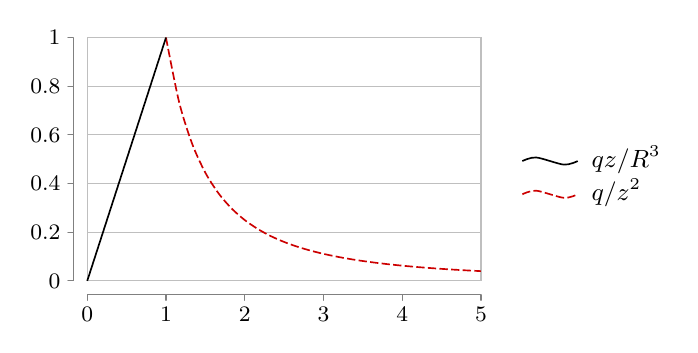
\begin{tikzpicture}
\datavisualization [scientific axes=clean,
                    y axis=grid,
                    visualize as smooth line/.list={inside,outside},
                    style sheet=strong colors,
                    style sheet=vary dashing,
                    inside={label in legend={text=$qz/R^3$}},
                    outside={label in legend={text=$q/z^2$}},
                    data/format=function
                    ]
data [set=inside] {
  var x : interval [0.0:1.0];
  func y = \value x;
}
data [set=outside] {
  var x : interval [1.0:5.0];
  func y = 1.0/(\value x*\value x);
};
\end{tikzpicture}

\section{DIVERGENCE AND CURL OF ELECTROSTATIC FIELDS}
\subsection{Field Lines, Flux and Gauss-s Law}

Equation \ref{eq:G01_electrostatic_field_continuous_vol} is the recipe for computing the electric \tit{field} of a charge distribution, then equation \ref{eq:G01_electrostatic_force} tells us what the \tit{force} on a charge $Q$ placed in this field will be. The integrals involved in computing $\vb{E}$ can be very difficult to calculate, even for relatively simple charge distributions. One then often exploits certain properties of the electric field by which the latter can be determined without an explicit calculation of the integral in \ref{eq:G01_electrostatic_field_continuous_vol}. 

Much can be understood about a vector field $\vb{E}$ by the values of its \tit{divergence} and \tit{curl}. There is indeed a general result of vector calculus -- Helmoltz's Theorem -- by which any vector field $\vb{A}$ that is sufficiently smooth and satisfying appropriate boundary conditions can be decomposed into the sum of a \tit{curl-free} ($\curl{\vb{A}}=\vb{0}$) field plus a \tit{divergence-free} ($\div{\vb{A}}=0$) field.     

$\vb{E}$ is a  \tit{curl-free} vector field and this is a consequence of 
\begin{itemize}
\item it being \tit{linearly} dependent on the source charges, so that a \tit{superposition principle} holds; 
\item it being directed \tit{radially} from any infinitesimal charge-carrying volume $d\tau$, so that integrating over a path that lies on a spherical surface centered on the source charge yields \tit{zero}; 
\item its \tit{magnitude} at any point $\vb{r}$ being a function of the distance of that point from any infinitesimal charge-carrying volume $d\tau$ located at $\vb{r}'$ ($\abs{\vb{E}(\vb{r})} = f(\abs{\vb{r} - \vb{r}'})$)\footnote{Note that the following demonstration does not require the field to decay by an inverse-square law as the electric field does.}. 
\end{itemize}

The reasoning to demonstrate that $\vb{E}$ is \tit{curl-free} goes as follows:
\begin{itemize}[-]
\item By Stokes theorem of vector calculus, given $\Gamma$ any closed curve and $\Sigma$ any closed surface bounded by  $\Gamma$, the \tit{line-integral} of $\vb{E}$ along $\Gamma$ (also called the \tit{circulation} of $\vb{E}$) equals the \tit{surface-integral} of $\curl{\vb{E}}$ (also called the \tit{flux of rotation}). 
\item Any closed path $\Gamma$ can be approximated to any precision degree by a curve made of an infinite sequence of steps where each step consists of an infinitesimal \tit{radial} displacement followed by a displacement along a spherical surface centered on the source charge $d\tau$ located at $\vb{r}'$. The latter type of displacement in each step \tbf{contributes nothing} to the line integral of $\vb{E}$, because the field is at right-angle with the path.
\item Given that only \tit{radial displacements} contribute to the line integral of $\vb{E}$ the latter must vanish on any closed path, since all outwardly directed displacements must be compensated by an equivalent amount of inwardly directed ones in order for the path to close.    
\item Due to the superposition principle, the vanishing of the \tit{circulation} thus holds for any field $\vb{E}$ and this in turn implies the vanishing of the \tit{flux of rotation}. The vanishing of the latter over the infinitely many surfaces bounded by an arbitrarily chosen curve $\Gamma$ clearly requires that $\curl{\vb{E}}=\vb{0}$.     
\end{itemize}
%\footnote{This is true also of fields generated by charges that are not static.}  % Griffiths - Electrodynamics / Electrostatics
%\include{Griffiths_02}	 % Griffiths - Electrodynamics / Potentials
%\include{Griffiths_03}	 % Griffiths - Electrodynamics / Electric Fields in Matter
%\include{Griffiths_04}	 % Griffiths - Electrodynamics / Magnetostatics
%\include{Griffiths_05}	 % Griffiths - Electrodynamics / Magnetic Fields in Matter
%\include{Griffiths_06}	 % Griffiths - Electrodynamics / Electrodynamics
%\include{Griffiths_07}	 % Griffiths - Electrodynamics / Conservation Laws
%\include{Griffiths_08}	 % Griffiths - Electrodynamics / Electromagnetic Waves
%\include{Griffiths_09}	 % Griffiths - Electrodynamics / Radiation
%\include{Griffiths_10}	 % Griffiths - Electrodynamics / Electrodynamics and Relativity
%\include{Griffiths_11}	 % Griffiths - Electrodynamics / Potentials and Fields
%\include{Griffiths_12}	 % Griffiths - Electrodynamics / Helmoltz Theorem

%\chapter{Jackson -- Maxwell Equations, Conservation Laws}
\label{ch:Jackson_06} 

\section{Maxwell Equations}

\begin{equation}
\begin{aligned}
\div{\vb{B}} &= 0\\
\curl{\vb{E}} + \frac{1}{c} \pdv{\vb{B}}{t} &= 0\\
\div{\vb{E}} &= 4 \pi \rho\\
\curl{\vb{B}} &= \frac{4 \pi}{c} \vb{J} + \frac{1}{c} \pdv{\vb{E}}{t}
\end{aligned}
\label{eq:maxwell}
\end{equation}


\section{Potentials}

$\vb{B}$ has a vanishing divergence, therefore a vector field $\vb{A}$ exists such that

\begin{equation}
\vb{B} = \curl{\vb{A}}
\label{eq:Adef}
\end{equation}

Substituting \ref{eq:Adef} in the second of Maxwell equations one gets

\begin{equation*}
\curl{\vb{E}} + \frac{1}{c} \pdv{\curl{\vb{A}}}{t} = 0
\end{equation*}

whence 

\begin{equation}
\curl{ \left( \vb{E} + \frac{1}{c} \pdv{\vb{A}}{t} \right)} = 0
\end{equation}

The expression enclosed in parentheses in the above equation implies that a scalar field $\phi$ exists such that 

\begin{equation}
\vb{E} + \frac{1}{c} \pdv{\vb{A}}{t} = - \grad{\phi}
\label{eq:phidef}
\end{equation}


Using the last equation in \ref{eq:maxwell} and a known theorem of vector calculus

\begin{align*}
\curl{\vb{B}} &= \curl{(\curl{\vb{A}})} \\
&= \grad{(\div{\vb{A}})} - \laplacian{\vb{A}} \\
&= \frac{4 \pi}{c} \vb{J} + \frac{1}{c} \pdv{\vb{E}}{t}
\end{align*}

while from \ref{eq:phidef}

\begin{align*}
\frac{1}{c} \pdv{\vb{E}}{t} = - \frac{1}{c} \pdv{\grad{\phi}}{t} - \frac{1}{c^2} \pdv[2]{\vb{A}}{t}  
\end{align*}

therefore

\begin{align*}
\grad{(\div{\vb{A}})} - \laplacian{\vb{A}} &= \frac{4 \pi}{c} \vb{J} + \frac{1}{c} \pdv{\vb{E}}{t} \\
&= \frac{4 \pi}{c} \vb{J} - \frac{1}{c} \pdv{\grad{\phi}}{t} - \frac{1}{c^2} \pdv[2]{\vb{A}}{t}  
\end{align*}

With the goal of arriving at two independent equations for $\phi$ and $\vb{A}$ we put the equation for $\vb{A}$ in the following form 

\begin{equation}
\begin{aligned}
\laplacian{\vb{A}} - \frac{1}{c^2} \pdv[2]{\vb{A}}{t} &= - \frac{4 \pi}{c} \vb{J} \\
&+ \grad{\left( \div{\vb{A}} + \frac{1}{c} \pdv{\phi}{t} \right)}
\label{eq:uglyA}
\end{aligned}
\end{equation}

Turning to the scalar potential $\phi$ and combining the third equation in \ref{eq:maxwell} with \ref{eq:phidef} we obtain 

\begin{equation}
\begin{aligned}
\div{\vb{E}} &=   4 \pi \rho \\
&= - \laplacian{\phi} - \frac{1}{c} \pdv{\div{\vb{A}}}{t}
\label{eq:uglyPhi}
\end{aligned}
\end{equation}

\section{Gauge transformations}
Equations \ref{eq:uglyA} and \ref{eq:uglyPhi} are interdependent: one cannot be solved without the other having been solved. They stem from equations \ref{eq:Adef} and \ref{eq:phidef}, where potentials were introduced (respectively $\vb{A}$ and $\phi$) to yield fields $\vb{B}$ and $\vb{E}$ that by construction satisfy two of the four Maxwell equations \ref{eq:maxwell} (the homogeneous ones). 
However, the equations \ref{eq:Adef} and \ref{eq:phidef} do not uniquely determine the potentials. Indeed, if 
$\vb{A}$ and $\phi$ satisfy the equations, the same is true of the potentials $\vb{A}'$ and $\phi'$ obtained with the following transformation

\begin{equation}
\begin{aligned}
\vb{A}  &\longrightarrow \: \vb{A}' = \vb{A} + \grad{\lambda(\vb{r}, t)} \\   
\phi    &\longrightarrow \: \phi' = \phi - \frac{1}{c} \pdv{\lambda(\vb{r}, t)}{t}   
\label{eq:gaugexform}
\end{aligned}
\end{equation}

where $\lambda(\vb{r}, t)$ is any scalar function of position and time.

\subsection{Lorenz gauge}

Imposing the following constraint (\textit{Lorenz gauge}) on the potentials $\phi$ and $\vb{A}$

\begin{equation}
\div{\vb{A}} + \frac{1}{c} \pdv{\phi}{t} = 0
\label{eq:lorenzgauge} % Yes this is from Lorenz, not from the other (Lorentz)
\end{equation}

amounts to apply the transformation \ref{eq:gaugexform} with $\lambda(\vb{r}, t)$ satisfying the following equation: 

\begin{align*}
\laplacian{\lambda} - \frac{1}{c^2} \pdv[2]{\lambda}{t} = \div{\vb{A}} + \frac{1}{c} \pdv{\phi}{t}
\end{align*}


As a result, one obtains two independent \textit{wave equations} governing the dynamics of $\phi$ and $\vb{A}$, where the \textit{source fields} $\rho$ and $\vb{J}$ appear in the respective inhomogeneous terms: 


\begin{equation}
\laplacian{\phi} - \frac{1}{c^2} \pdv[2]{\phi}{t} = - 4 \pi \rho
\label{eq:PhiWave}
\end{equation}

\begin{equation}
\laplacian{\vb{A}} - \frac{1}{c^2} \pdv[2]{\vb{A}}{t} = - \frac{4 \pi}{c} \vb{J} 
\label{eq:AWave}
\end{equation}


\subsection{Coulomb gauge}

 

 




    % J.D. Jackson -- Classical Electrodynamics, 2nd Edition
%\include{Jackson_07}    % J.D. Jackson -- Classical Electrodynamics, 2nd Edition

%\include{Jackson_11}    % J.D. Jackson -- Classical Electrodynamics, 3rd Edition
%\include{Jackson_12}    % J.D. Jackson -- Classical Electrodynamics, 3rd Edition

%\include{Franklin_02}   % J. Franklin -- Advanced Mechanics and General Relativity
%\include{Franklin_03}   % J. Franklin -- Advanced Mechanics and General Relativity
%\include{Franklin_04}   % J. Franklin -- Advanced Mechanics and General Relativity
%\include{Franklin_05}   % J. Franklin -- Advanced Mechanics and General Relativity
%\include{Franklin_06}   % J. Franklin -- Advanced Mechanics and General Relativity

%\include{Landau_01}	 % L.D. Landau, E.M. Lifshitz -- Teoria dei Campi
%\include{Landau_02}	 % L.D. Landau, E.M. Lifshitz -- Teoria dei Campi

%\include{Jackson_13}	 % J.D. Jackson -- Classical Electrodynamics, 3rd Edition
%\include{Jackson_14}	 % J.D. Jackson -- Classical Electrodynamics, 3rd Edition
%\include{Jackson_15}	 % J.D. Jackson -- Classical Electrodynamics, 3rd Edition
%\include{Jackson_16}	 % J.D. Jackson -- Classical Electrodynamics, 3rd Edition

%\include{MTWheeler_02}	 % C.W. Misner, K.S. Thorne, J.A. Wheeler -- Gravitation
%\include{MTWheeler_03}	 % C.W. Misner, K.S. Thorne, J.A. Wheeler -- Gravitation
%\include{MTWheeler_04}	 % C.W. Misner, K.S. Thorne, J.A. Wheeler -- Gravitation

%\include{Landau_03}	 % L.D. Landau, E.M. Lifshitz -- Teoria dei Campi
%\include{Landau_04}	 % L.D. Landau, E.M. Lifshitz -- Teoria dei Campi
%\include{Landau_05}	 % L.D. Landau, E.M. Lifshitz -- Teoria dei Campi
%\include{Landau_06}	 % L.D. Landau, E.M. Lifshitz -- Teoria dei Campi
%\include{Landau_07}	 % L.D. Landau, E.M. Lifshitz -- Teoria dei Campi
%\include{Landau_08}	 % L.D. Landau, E.M. Lifshitz -- Teoria dei Campi
%\include{Landau_09}	 % L.D. Landau, E.M. Lifshitz -- Teoria dei Campi

%\appendixpage
%\appendix
\chapter{Tensors}
\label{ch:Tensors} 

\section{Vector Algebra}
For the sake of fixing notation, let $\{\vu{i}, \vu{j}, \vu{k}\}$ be an \textit{orthonormal} basis of unit vectors in three-dimensional space, and the following a list of all possible scalar products of basis vectors. 
  
\begin{equation}
\begin{aligned} 
\vu{i}\vdot \vu{i} &= \vu{j} \vdot \vu{j} = \vu{k} \vdot \vu{k} = 1 \\ 
\vu{i} \vdot \vu{j} &= \vu{j} \vdot \vu{k} = \vu{k} \vdot \vu{i} = 0 
\label{eq:basis_dot_products}
\end{aligned}
\end{equation}

For a \textit{right-handed} basis, the following is a list of all possible \textit{vector} products of basis vectors.
  
\begin{equation}
\begin{aligned} 
\vu{i} \cross \vu{i} &= \vu{j} \cross \vu{j} = \vu{k} \cross \vu{k} = 0 \\ 
\vu{i} \cross \vu{j} &= \vu{k} = - \vu{j} \cross \vu{i}\\
\vu{j} \cross \vu{k} &= \vu{i} = - \vu{k} \cross \vu{j}\\
\vu{k} \cross \vu{i} &= \vu{j} = - \vu{i} \cross \vu{k}
\label{eq:basis_vector_products}
\end{aligned}
\end{equation}





\backmatter%%%%%%%%%%%%%%%%%%%%%%%%%%%%%%%%%%%%%%%%%%%%%%%%%%%%%%%
%%%%%%%%%%%%%%%%%%%%%%%%% referenc.tex %%%%%%%%%%%%%%%%%%%%%%%%%%%%%%
% sample references
% 
% Use this file as a template for your own input.
%
%%%%%%%%%%%%%%%%%%%%%%%% Springer-Verlag %%%%%%%%%%%%%%%%%%%%%%%%%%

%
% BibTeX users please use
% \bibliographystyle{}
% \bibliography{}
%
% Non-BibTeX users please use
\begin{thebibliography}{99.}
%
% and use \bibitem to create references.
%
% Use the following syntax and markup for your references
%
% Monograph
\bibitem{Griffiths_4th} D.J. Griffiths (2017)
Introduction to Electrodynamics. Cambridge University Press, Cambridge

% Monograph
\bibitem{Felsager_1981} B. Felsager (1981)
Geometry, Particles and Fields. Odense University Press

% Monograph
\bibitem{BudakFomin_1973} B.M. Budak, S.V. Fomin (1973)
Multiple Integrals, Field Theory and Series. Mir Publishers, Moscow

% Monograph
\bibitem{Postnikov_II_1982} Mikhail Postnikov (1982)
Lectures in Geometry, Semester II. Linear Algebra and Differential Geometry. Mir Publishers, Moscow

\end{thebibliography}

\printindex

%%%%%%%%%%%%%%%%%%%%%%%%%%%%%%%%%%%%%%%%%%%%%%%%%%%%%%%%%%%%%%%%%%%%%%

\end{document}





